%%
%% Copyright 2007-2019 Elsevier Ltd
%%
%% This file is part of the 'Elsarticle Bundle'.
%% ---------------------------------------------
%%
%% It may be distributed under the conditions of the LaTeX Project Public
%% License, either version 1.2 of this license or (at your option) any
%% later version.  The latest version of this license is in
%%    http://www.latex-project.org/lppl.txt
%% and version 1.2 or later is part of all distributions of LaTeX
%% version 1999/12/01 or later.
%%
%% The list of all files belonging to the 'Elsarticle Bundle' is
%% given in the file `manifest.txt'.
%%

%% Template article for Elsevier's document class `elsarticle'
%% with numbered style bibliographic references
%% SP 2008/03/01
%%
%%
%%
%% $Id: elsarticle-template-num.tex 164 2019-01-14 09:57:55Z rishi $
%%
%%
%%\documentclass[preprint,12pt]{elsarticle}

%% Use the option review to obtain double line spacing
%% \documentclass[authoryear,preprint,review,12pt]{elsarticle}

%% Use the options 1p,twocolumn; 3p; 3p,twocolumn; 5p; or 5p,twocolumn
%% for a journal layout:
%% \documentclass[final,1p,times]{elsarticle}
%% \documentclass[final,1p,times,twocolumn]{elsarticle}
%% \documentclass[final,3p,times]{elsarticle}
\documentclass[final,3p,times,twocolumn]{elsarticle}
%% \documentclass[final,5p,times]{elsarticle}
%%%\documentclass[final,5p,times,twocolumn]{elsarticle}

%% For including figures, graphicx.sty has been loaded in
%% elsarticle.cls. If you prefer to use the old commands
%% please give \usepackage{epsfig}

%% The amssymb package provides various useful mathematical symbols
\usepackage{amssymb}
%% The amsthm package provides extended theorem environments
%% \usepackage{amsthm}
\usepackage{amsmath}
\usepackage{indentfirst}
\usepackage{epsfig}
\usepackage{ulem}
% \usepackage{epstopdf}
\usepackage{listings}
\usepackage{subfig}
\usepackage{lipsum}
\usepackage{color}
\usepackage{soul}
%\usepackage[lined,algonl,ruled]{algorithm2e}
% \usepackage{subfigure}
\usepackage{graphicx}
\usepackage[T1]{fontenc}
\newcommand{\secref}[1]{Section \ref{#1}}
\newcommand{\figref}[1]{Figure \ref{#1}}
\newcommand{\tabref}[1]{Table \ref{#1}}
\newcommand{\equref}[1]{Equation (\ref{#1})}
% \renewcommand{\algorithmicrequire}{\textbf{Input:}}
% \renewcommand{\algorithmicensure}{\textbf{Output:}}
\newcommand{\KZ}[1]{\textcolor{red}{[Kenny: #1]}}
%\newcommand{\JY}[1]{\textcolor{blue}{[Jinyi: #1]}}
\newcommand{\KQ}[1]{\textcolor{red}{#1}}
\lstset{
  captionpos=b,
  tabsize=2,
  % numbers=left,
  % numberstyle=\tiny,
  % numbersep=5pt,
  breaklines=true,
  showstringspaces=true,
  basicstyle=\small,
  frame=none,
  emph={label},
  escapechar=* % Escape to LaTeX between |...|
}
%% The lineno packages adds line numbers. Start line numbering with
%% \begin{linenumbers}, end it with \end{linenumbers}. Or switch it on
%% for the whole article with \linenumbers.
%% \usepackage{lineno}

\journal{Computers in Biology and Medicine}

\begin{document}

\begin{frontmatter}

%% Title, authors and addresses

%% use the tnoteref command within \title for footnotes;
%% use the tnotetext command for theassociated footnote;
%% use the fnref command within \author or \address for footnotes;
%% use the fntext command for theassociated footnote;
%% use the corref command within \author for corresponding author footnotes;
%% use the cortext command for theassociated footnote;
%% use the ead command for the email address,
%% and the form \ead[url] for the home page:
%% \title{Title\tnoteref{label1}}
%% \tnotetext[label1]{}
%% \author{Name\corref{cor1}\fnref{label2}}
%% \ead{email address}
%% \ead[url]{home page}
%% \fntext[label2]{}
%% \cortext[cor1]{}
%% \address{Address\fnref{label3}}
%% \fntext[label3]{}

\title{Layout-aware Information Extraction from Semi-structured Medical Images}

%% use optional labels to link authors explicitly to addresses:
%% \author[label1,label2]{}
%% \address[label1]{}
%% \address[label2]{}

\author[sjtu]{Kangqi Luo}
\author[sjtu]{Jinyi Lu}
\author[sjtu]{Kenny Q. Zhu\corref{cor1}}
\ead{kzhu@cs.sjtu.edu.cn}

\author[az]{Weiguo Gao}
\author[az]{Jia Wei\corref{cor1}}
\ead{jenny.wei@astrazeneca.com}
\author[az]{Meizhuo Zhang}

\address[sjtu]{Shanghai Jiao Tong University, 800 Dongchuan Road, Shanghai 200240, P.R. China}
\address[az]{AstraZeneca China, 199 Liangjing Road, Shanghai 201203, P.R. China}

\cortext[cor1]{Corresponding authors.}

\begin{abstract}
\st{
Digitizing paper documents and extracting structured information is an
important part of information retrieval and knowledge discovery.
Optical character recognition (OCR) has been widely used
in this task, and achieved promising results on textual documents
%and promising results have been achieved in applying OCR to textual documents,
such as books and reports.
For the ultimate goal of building electronic medical records,
the textual information embedded in the medical image
contains rich structured knowledge of the particular patient.
% For %semi-structured
% medical images that combine graphics and words,
However, due to the discontinuity of text flows,
%extraction of useful textual information is difficult
extracting structured textual data from medical images becomes more challenging.
}
\KQ{
Textual information embedded in the medical image
contains rich structured information about the medical condition of a patient.
This paper aims at extracting structured textual information from semi-structured medical images.
Given the recognized text spans of an image preprocessed by
optical character recognition (OCR),
due to the spatial discontinuity of texts spans
as well as potential errors brought by OCR,
the structured information extraction becomes more challenging.
}
In this paper, we propose a
domain-specific language, called ODL, which allows users to describe
the value and layout of text data contained in the images.
Based on the value and spatial constraints described in ODL,
the ODL parser
\st{parses the raw OCR output of the medical image into a parse tree, and}
associates values found in the image with the data structure in the
ODL description, while conforming to the aforementioned constraints.
\st{
Robustness is the major advantage during this parsing process,
as the parser doesn't rely on carefully annotated bounding boxes
of structured data in the medical image,
and is able to tolerate or even automatically correct some of the errors
introduced by OCR.
Compared with baseline methods in the same task,
our ODL parser shows the better tolerance of positional variances between
images, and consistently outperforms existing approaches in terms of
extraction accuracy.
}
\KQ{
We conduct experiments on a dataset consisting of real medical images,
our ODL parser consistently outperforms existing approaches in terms of
extraction accuracy,
which shows the better tolerance of incorrectly recognized texts,
and positional variances between images.}
This accuracy can be further improved by learning from a few manual corrections.

\end{abstract}

\begin{keyword}
%% keywords here, in the form: keyword \sep keyword
information extraction \sep
medical images \sep
electronic medical records \sep
domain-specific language \sep
spatial layout \sep
optical character recognition

%% PACS codes here, in the form: \PACS code \sep code

%% MSC codes here, in the form: \MSC code \sep code
%% or \MSC[2008] code \sep code (2000 is the default)

\end{keyword}

\end{frontmatter}

%% \linenumbers
\section{Introduction}
\label{sec:intro}

% Part 1: Text IE, scenarios, OCR
% What is text information extraction?
Information extraction is the task of automatically extracting information
or knowledge from unstructured or semi-structured documents.
In the domain of image processing,
the task of textual information extraction (TIE)
is automatically detecting and recognizing texts from given images.
% where is it used?
TIE is applied in a large variety of image categories,
such as printed books, newspapers, digital drawings,
or even more general images~\cite{jung2004text}.
% What's the kernel technique?
Optical character recognition (OCR) is the popular approach to solve TIE,
turning images of printed text into machine encoded texts.
OCR is a hot research topic in recent years, and the performance is promising
on plain-text-based images, such as novels and reports.
For example, Tesseract~\cite{smith2007overview},
one of the most popular open source multilingual recognizers,
achieved an error rate of 3.72\% for recognizing English words
and 3.77\% for simplified Chinese characters\cite{smith2009adapting}.
Based on the exclusive use and high accuracy of OCR,
the Google Books~\cite{vincent2007google} and Gutenberg Project~\cite{lebert2008project}
have scanned a large number of printed books
and converted into text for free and open access.

\begin{figure}[!htb]
\centering
\subfloat[ECG]{
\label{fig:medicalimage:ecg}
\epsfig{file=figure/ECG.eps, width=0.5\columnwidth}
}
% % \hfill
% \subfloat[X-RAY]{
% \label{fig:medicalimage:xray}
% \epsfig{file=figure/X-RAY.eps, width=0.4\columnwidth}
% }
% \hfill
\subfloat[MRI]{
\label{fig:medicalimage:mrt}
\epsfig{file=figure/MRI.eps, width=0.4\columnwidth}
}
% \subfloat[EEG]{
% \label{fig:medicalimage:eeg}
% \epsfig{file=figure/EEG.eps, width=0.4\columnwidth}
% }
\caption{Examples of medical images.}
\label{fig:med-image-example}
\end{figure}


% Part 2: Medical imaging, example image, raw OCR result (text + layout information)
% What's medical image, why important?
Due to ever evolving hardware and software, many medical images
such as electro-cardio graphs (ECGs), magnetic resonance imaging (MRI),
X-ray or ultrasound images are directly printed and stored in hard copy formats.
Medical images shown in \figref{fig:med-image-example}
contain a mix of graphics and text,
which include technical settings of the hardware used,
test measurements and simple diagnoses.
% TODO: why growing demand?
In order to build the manageable electronic medical records for patients,
there has been a growing demand for extracting such text-based
medical information from these medical images.
% What's the exmaple, and what's in the OCR output?
Given the ECG image in \figref{fig:running-ecg} as the running example,
existing OCR softwares are able to produce texts with spatial layout information,
indicating the positions of each recognized text in the image.
\figref{fig:running-xml} shows the raw OCR result produced by Tesseract,
where recognized texts are organized in the form of XML hierarchy of spans,
and we call them ``text boxes'' throughout this paper.
Texts are stored only in leaf text boxes,
and the layout information of each box is represented by
the coordinates (left, top, right, bottom) of its bounding box.
We use the term ``bounding box'' and ``zone'' interchangeably in this paper.
% TODO: Mention OCR error here??
It's worth mentioning that OCR softwares may generate incorrect texts.
for example, the original text ``Vent. rate'' in the image
is incorrectly recognized as ``Vcnt. rule'',
also ``63 bpm'' is recognized as ``53 bpm''.

\begin{figure}[ht]
\centering
\epsfig{file=figure/running_ECG.eps, width=0.9\columnwidth}
\caption{An ECG with interesting text areas marked by red ovals.}
\label{fig:running-ecg}
\end{figure}

% \begin{figure}[ht]
% \centering
% \subfigure[]{
% \label{fig:subfig:a}
% \begin{minipage}[b]{0.2\textwidth}
%\newsavebox{\firstlisting}
%\begin{lrbox}{\firstlisting}% Store first listing
%\begin{lstlisting}
%<p class='ocr_par' dir='ltr'>
%   <span class='ocr_line' id='line_2'>
%       <span class='ocrx_word' id='word_6'>Vent.</span>
%       <span class='ocrx_word' id='word_7'>rate</span>
%       <span class='ocrx_word' id='word_8'>65</span>
%       <span class='ocrx_word' id='word_9'>bpm</span>
%   </span>
%   <span class='ocr_line' id='line_3'>
%       <span class='ocrx_word' id='word_14'>PR</span>
%       <span class='ocrx_word' id='word_15'>interval</span>
%       <span class='ocrx_word' id='word_16'>162</span>
%       <span class='ocrx_word' id='word_17'>ms</span>
%   </span>
%    ...
%</p>
%\end{lstlisting}
%\end{lrbox}
% \end{minipage}
% }
% \hspace[1in]
% \subfigure[]{
% % \label{fig:subfig:b}
% % \begin{minipage}[b]{0.2\textwidth}
\newsavebox{\secondlisting}
\begin{lrbox}{\secondlisting}
% \tiny
\begin{lstlisting}[basicstyle=\tiny,]
<p class="ocr_par" title="box 263 33 444 119">
   <span class="ocr_l" title="box 264 33 336 45">
       <span class="ocrx_w" title="box 264 33 299 45">Vcnt.</span>
       <span class="ocrx_w" title="box 308 34 336 45">rule</span>
   </span>
   <span class='ocr_l'>
       <span class="ocrx_w" title="box 264 51 283 64">PR</span>
       <span class="ocrx_w" title="box 291 51 346 64">Interval</span>
       <span class="ocrx_w" title="box 389 52 411 64">140</span>
       <span class="ocrx_w" title="box 420 55 439 64">ms</span>
   </span>
   ...
   </span>
</p>
<p class="ocr_p" dir="ltr">
   <span class="ocr_l">
       <span class="ocrx_w" title="box 396 33 411 45">53</span>
       <span class="ocrx_w" title="box 420 33 449 48">bpm</span>
   </span>
</p>
\end{lstlisting}
\end{lrbox}
% % \end{minipage}
% }

% \KZ{\figref{fig:ocrre} is output from what software? Tesseract?}
\begin{figure*}[th]
%\subfloat[Image From Printer1]{
%\label{fig:ocrresub:a}
%\scalebox{0.8}{\usebox{\firstlisting}}}
%\hfill
%\subfloat[Image From Printer2]{
\scalebox{1.6}{\usebox{\secondlisting}}
% \label{fig:ocrre}
\caption{A fragment of raw OCR results for ECG with layout information.}
%\caption{Simplified OCR Results in XML for an ECG with Layout Information}
%\label{fig:ocrresub:b}
\label{fig:running-xml}
\end{figure*}

% \lipsum[2]



% Part 3: Goal of this paper: structured information (kv pair) extraction
%         Challenge: hard to write wrapper (professional, not friendly)
%                    noisy information & OCR error
%         direct approach: zonal approaches
%         weakness: error propagation
% kernel: structure --> pure OCR (text, regex based approach) is not reliable: not in a same box
% ZOI approach: zonal / page layout: inaccurate position (between diff. figures), error propagation

% What's the final goal?
Apart from scanning the images into digital formats,
extracting the structured textual knowledge is more important for
building electronic medical records.
% Using examples to illustrate.
For example in \figref{fig:running-ecg},
we would like to extract the attribute-value pairs
(e.g., \textit{Vent. rate = 63 bpm}) and possibly other values such as
date (e.g., \textit{18-Nov-2010}) and time (e.g., \textit{9:13:02}),
since those values endow us with information of the particular patient.
% Informally define the task
% Obviously, raw OCR results didn't explicitly encode such structured knowledge,
Since discovering structured knowledge is beyond the scope of the OCR techniques,
the goal of this work is to provide a systematic solution,
which enables users to easily specify the data of interest in the images,
and automatically extract the corresponding textual values from raw OCR results.

There are some naive solutions for this information extraction task.
% Naive approach 1: regex matching
The first approach is to write regex expressions for each data to be extracted,
and apply them to different text boxes of the OCR result.
For example, using \textit{``Vent\textbackslash . rate .* bpm''}
to capture the target bpm value.
However, this approach suffers from two major problems.
First and obviously,
incorrect recognized texts lead to mismatches of regex rules.
Second, the hierarchical layout of OCR results are
not always organized in a human-readable manner.
For example in \figref{fig:running-xml}, the text ``Vcnt. rule'' and ``53 bpm''
are not automatically combined into the same text box, but are rather far apart.
In fact, the hierarchical layout is sensitive to many factors,
including color, contrast, accidental spots on the prints, or the angle of the scanner camera.
In this case, text-based regex rules are not well suited for medical images.
Besides, writing regex rules is too ad-hoc and non-trivial for end users.

% Naive approach 2: ZOI based
The second approach is more straightforward:
the user first annotates all the target zones of each desired data,
then simply conducts OCR on each fragment of images.
Though intuitive and easy to implement,
this approach highly relies on the the accuracy of carefully annotated zones,
either too larger or too smaller will affect the local OCR results.
% TODO: why?? I don't know.
In addition, there exists slight positional variations of target zones
between two images, even if they share the same format.
Therefore, the user have to annotate zones for every individual image,
which is tedious and labour intensive.

% Naive approach 3: page layout
Another alternative solution involves the page layout analysis technique~\cite{o1993document},
which includes identifying and organizing the textual regions
in the scanned image of a text document.
\figref{fig:running-page-layout} shows the page layout result of the running example.
In particular, the technique first segments textual zones (blue blocks) from
non-textual zones and arrange them in their original order,
then detects individual text unit (red lines under texts) in each zone.
% Then in order to analyze the logical roles of the text zones
% (titles, captions, footnotes, etc.), logical layout analysis
% is used for labeling the semantics of the text zones.
Page layout analysis is mainly used for analyzing the semantics of text zones
for plain text image documents,
and it encounters two problems when applied to this task.
% When applied to structured TIE on medical images,
% this technique encounters two problems.
First, it is based on the strong assumption that images of the same format
share the same structure of page layout result.
Noises in the image will affect the page layout result and
eventually generate totally error textual information.
Second, users must implement an addition wrapper to describe the location
(which texts in which regions) of each desired data.
This step highly depends on the detail result of page layout,
and writing such wrapper is almost intractable
for common users without expert knowledge.
% The page layout analysis technique is used to determine where the text
% resides on a page ,
% % By using page layout analysis technique, the hierarchy of physical components
% % can be generated and to match with the hierarchy of logical components, which
% % is predefined.
% The problem with applying
% such technique on medical images is that it creates so much noises
% that performance is ultimately affected.
% For medical images like ECG, useful information is often
% found in the small components of the image, while most of the images are
% regarded as noises.
% % check paper and more description, weakness, ref
\begin{figure}[ht]
\centering
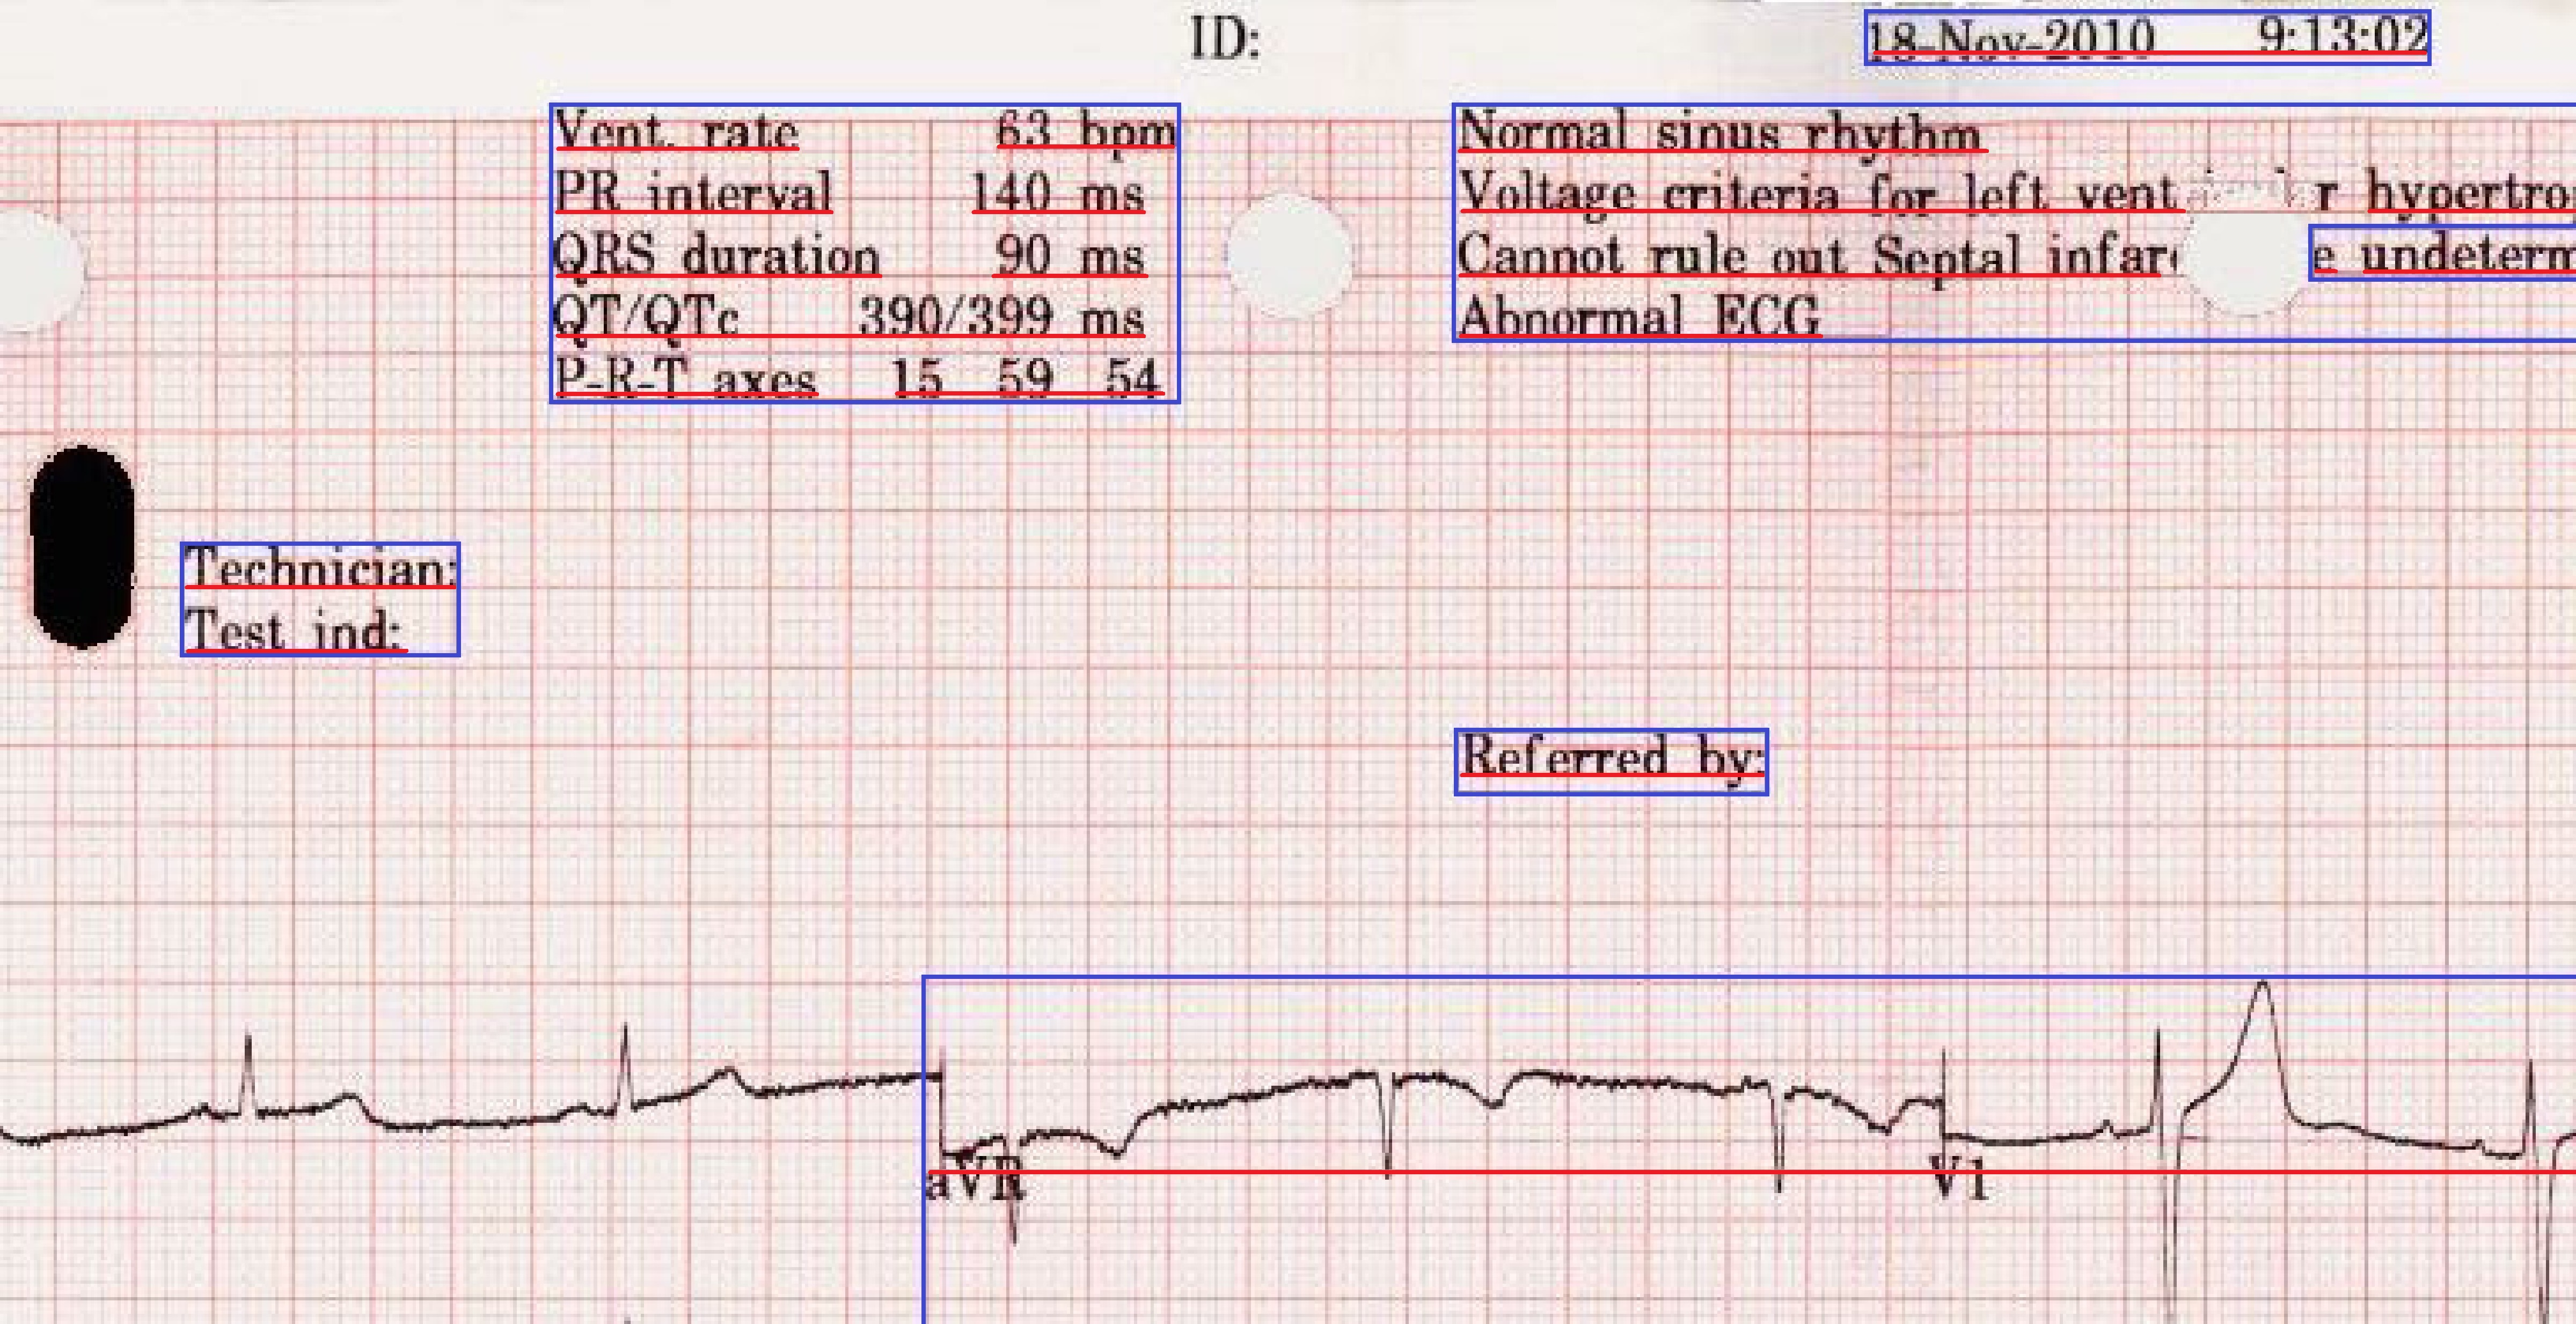
\epsfig{file=figure/page_layout.jpg, width=0.9\columnwidth}
\caption{Example result of page layout analysis.}
\label{fig:running-page-layout}
\end{figure}

% Part 4: Our approach: ODL based (in fact we are writing a parser)
%         user-friendly;
%         present spatial information via element order (LR, UD) and rough spatial constraints, without too precise position
%         What's more: support error prompt and automatic correction based on OCR info & human correction.
% to solve: treat as an alignment problem: find the best alignment between var and box,
%       satisfying both data-level and spatial-level constraints.
% Challenge: How to measure the spatial-level fitness without hard code position information?
% Our approach: DSL-based, 3 advantages:
%    1. user-friendly: simple syntax to describe what's in the image, and what's the data-of-interest. all need: following left-to-right and top-to-bottom style.
%    2. robust and efficient alignment (fuzzy): leverage relative position and rough coordinates defined in ODL tolerant position delta
%    3. correction model: automatic made correction based on OCR and human feedbacks, and prompt errors to easily tell user what's wrong.

% 1. avoid what, our intuition is?
In order to attack the limitations of the above approaches,
We propose a domain-specific language for describing and extracting
structured textual information from the raw OCR data of medical images.
We call it OCR description language, or ODL in short.
The ODL parser then parses the raw OCR data
of the medical images according to the description,
and extracts structured textual data in a tree shape.
The ODL based solution has three major advantages.
% adv 1. user-friendly
First, compared with the previous methods, ODL is more user-friendly.
%Instead of writing ad-hoc wrappers,
Borrowing the syntax from PADS~\cite{fisher2005pads},
an ad-hoc data processing language,
ODL provides a concrete syntax which allows users to easily define
fixed strings and variables to be extracted,
customize compositions for better organizing structured data,
apply value constraints on variables, and rough spatial constraints on structures.
% adv 2. layout-aware
Second, the syntax of ODL is layout-aware.
Besides the explicit description of the bounding boxes of individual data,
ODL also implies the relative layout between different data elements,
which is based on the left-to-right and top-to-bottom data description manner.
Those rich layout information support the effectiveness of the ODL parser.
% so that ODL implies the relative layout between different elements.
% adv 3. robust and efficient alignment
Third, the parsing process of ODL is robust.
Intuitively, the process aims at finding the best alignments
between the data defined in ODL and the text boxes of the raw OCR result,
satisfying both value constraints,
spatial constraints and their relative layouts.
The fuzzy matching strategy is applied to tolerate
or even automatically correct recognition errors brought by OCR,
as well as slight layout variances between images.
Therefore, neither carefully annotated zones nor
perfect OCR recognitions are required in the extraction step.
% % adv 3. automatic correction
% Third, the extraction results of ODL can be further
% improved by automatic correction.
% ODL is able to detect imperfect alignments via
% string mismatches or constraint violations,
% and then prompts the user to manually correct prominent parsing errors.
% These manual corrections serve as incremental annotations,
% which update the fuzzy matching strategy, and produce better extraction results.

% Or: 1. user friendly; 2. rich spatial semantics (implicit, explicit); 3. fuzzy


% Part 5: In summary, bullets.
In summary, this paper makes three main contributions.
\begin{enumerate}
\item We design a declarative spatial data description language
for describing both spatial and value constraints in medical images,
which can be used to automatically generate parsers for
structured information extraction from these images.
The syntax of ODL can be generalized to
%textual information extraction on
the other image domains (\secref{sec:syntax});
\item We propose a robust ODL parser,
which builds the association between the text boxes from raw OCR results
and the corresponding description in ODL.
During the parsing phase, the parser is able to tolerate
the noises and errors brought by OCR recognition,
as well as inaccurate bounding boxes of input description (\secref{sec:parsing});
\item We conduct preliminary experimental studies of
structured information extraction on real ECG dataset.
The end-to-end evaluation result shows that our ODL based solution
consistently outperforms existing approaches.
Besides, the extraction accuracy further increases by 2\%,
given only a few number of manual corrections.
(\secref{sec:eval}).
\end{enumerate}


\section{Technical Specification}
\label{sec:algo}

\begin{figure*}[th]
\centering
\epsfig{file=pic/SystemOverview2.eps,width=1.8\columnwidth}
\caption{System Overview}
\label{fig:sys}
\end{figure*}

Figure \ref{fig:sys} shows the block diagram of our system.
As the input of the system, the web page is first parsed by 
a HTML parser\cite{winista} to obtain a complete DOM representation.
Then the title classifier attempts to recognize the page title.
If it is a ``top-$k$ like'' title, 
the classifier outputs the list size (the number $k$) 
and a set of possible concepts mentioned in the title.
With the number $k$, the candidate picker extracts all lists of size $k$ 
from the page body as candidate lists. Only one of them will be the actual
list of interest. With the concept set, 
the top-$k$ ranker can score each candidate list and pick the best one 
as the ``top-$k$'' list.  Finally the content processor  
analyzes the list content and extracts the entity names and attributes. 
%and conceptualize the main entities in the list
%as well as their attributes, if any. 

\subsection{Title Classifier}
\label{sec:title}

The title of a web page (string enclosed in {\tt<title>} tag) helps us
identify a top-$k$ page.  There are several reasons for us to utilize
the page title to recognized a top-$k$ page.  First, for most cases,
page titles serve to introduce the topic of the main body.  Second,
while the page body may have varied and complex formats, top-$k$ page
titles have relatively similar structure.  Also, title analysis is
lightweight and efficient. If title analysis indicates that a page is
not a top-$k$ page, we chose to skip this page.
This is important if the system has to scale to billions of web pages.

\begin{figure}
\centering
\epsfig{file=pics/pageTitle2.eps,width=0.9\columnwidth}
\caption{A Sample Top-K Title}
\label{fig:title}
\end{figure}

%We now discuss what a top-$k$ title should look like.
%In general, a top-$k$ title represents the topic of a top-$k$ list.
Figure \ref{fig:title} shows a typical top-$k$ title.  Note that the title
may contain multiple segments, and usually only one segment describes
the topic or concept of the list.  In addition to the value of $k$
(e.g, 10) and the head concept (e.g, ``podcasts''), a top-$k$ title
may include some other elements, such as the ranking criteria (e.g,
``top'', ``most memorable'', etc.) and other modifiers (e.g, ``.net
Awards'' and ``2011'').

\ZZX{
Note that a web page with a top-$k$ title may not contain a top-$k$ list.
A typical case is shown in Figure \ref{fig:slideshow}. Here the top-$k$ list
is divided into multiple interlinked pages, instead of being on a single page.
Extracting such lists requires that all relevant pages are in
the corpus and are properly indexed which increases the cost of the solution
significantly. Base on our observations, such multi-page top-$k$ lists
account for about 5\% of the total number of top-$k$ lists on the web,
we therefore choose to ignore this type of pages in this paper.
%additional crawling (because it is not
%certain that each of the page is in the web corpus) and it is too
%costly given that we need to handle billions of pages already.
}

We build a classifier to recognize top-$k$ titles.
Specifically, we train a Conditional Random Field (CRF)
\cite{CRFLafferty} model from a labeled dataset of both
positive titles and negative titles (negative titles also contain a
number).  We use lexical features such as {\em word}, {\em lemma}, and
{\em POS tag}\cite{santorini1990part} to form the basic feature set.  The classifier also
returns additional information such as the list size $k$ and a set of
concepts (recorded by a knowledge base such as Probase)
which are mentioned in the title.
\ZZX{We prefer to optimize the classifier for higher recall rather
than precision at this step, because some false positives pages,
which cannot be recognized through titles alone,
can be easily filtered out by validating against other properties
during the List Extraction phase.}
%
%Since we have additional mechanisms that help us filter out
%false positives pages (i.e, pages that are wrongly recognized as
%top-$k$ pages), we optimize the classifier for getting higher recall.
%\KZ{What additional mechanism?}

\begin{figure}
\centering
\epsfig{file=pics/page4.eps,width=0.8\columnwidth}
\caption{A Slide-show Page Snapshot\cite{TopFootball}}
\label{fig:slideshow}
\end{figure}

\subsubsection{The CRF model}
We convert the problem of recognizing top-$k$ titles to the problem of
recognizing the number $k$ in a top-$k$ context. For example, in
Figure \ref{fig:title}, ``10'' is the $k$ in the top-$k$ context,
while ``2010'' is not a $k$ even though it is also a number.

We consider the ``$k$ recognition task'' as a sequence labeling
problem: Each word in the title is considered a token in a sequence,
and is either $k$ or {\em not k}.
%The \emph{TRUE} label means the corresponding token is the $k$, and
%the title sequence is therefore recognized as a top-$k$ title.
CRF is well suited to such tasks.
The main idea of CRF is to calculate the
conditional probability of the whole label sequence given the
observation sequence.  We define $X=(X_{1}, X_{2}, X_{3}, ..., X_{n})$ as
a word sequence of length $n$, and $Y=(Y_{1}, Y_{2}, Y_{3}, ..., Y_{n})$
as a label sequence, where $Y_{i} \in \{TRUE, FALSE\}$.  The CRF model
calculates the conditional distribution $P(Y|X)$, and then selects the
$Y$ that maximizes the probability.

We use the linear chain as the undirected statistical graphical model,
which is based on the assumption that each label $Y_{i}$ only depends on
its immediate neighbors ($Y_{i+1}$ and $Y_{i-1}$).
For linear chain CRF, the conditional probability can be calculated as:
\begin{equation*}
    P(Y|X)=\frac{1}{Z(x)}\exp(\sum_{i=1}^{n}\sum_{j=1}^{m}\lambda_{j}f_{j}(y_{i-1},y_{i},x,i))
\end{equation*}
where $Z(x)$ is a normalization factor, $f_{j}$ is one of the $m$
functions that describes a feature, and $\lambda_{j}$ is the feature
weight to be trained.
To build an effective CRF model, we need to collect training data and
design a feature set, which is discussed below.

%We can build an undirected graph $G(V,E)$ to represent each $Y_{i} \in Y$
%according to the independency relations
%(in other words, if $Y_{i}$ and $Y_{j}$ depend on each other,
%there is an edge connecting the two nodes).
%Therefore, the overall probability $P(Y|X)$ is equal to
%the product of the potential functions of all the maximal cliques in $G(V,E)$.


%For web titles,
%The structure of the label sequence can be an arbitrary undirected graph,
%which is different from hidden Markov model\cite{HMMBaum}.
%For title recognition, the graph of interest is linear chain.
%
%
%Since in normal NLP tasks (including the title classifier in our system), the graph of interest is usually a linear chain. We will focus on this model in the following discussion.
%
%, or CRF\cite{CRFLafferty},
%is a probabilistic model based on undirected graphs.
%
%
%We can convert the original problem of Title Classifier
%into to a $k$ recognition task,
%The task is to find a proper number word in title,
%of which the context conveys a top-$k$ topic.
%
%
%Therefore the task becomes a sequence segmentation problem:
%each word in the title is a token in sequence to be assigned


\subsubsection{Creating a training dataset}
\label{sec:titleDataSet}
Creating a large, high quality training dataset is costly. The
challenge mainly lies in collecting positive cases, as top-$k$ pages
are sparse on the web (approx. 1.4\textperthousand{} of total web pages, see
Section \ref{sec:eval}). Filtering out pages without a number in
the title narrows our candidates down, but the number of candidates
is still massive.
%Although narrowing down the target to those whose titles contain at
%least a number, it is still difficult to manually collect enough
%positive cases.
In our approach, we first tokenize the titles to add POS
tags, and then we adopt the following simple rules to identify
or create positive training samples.
\begin{itemize}
\item \textbf{``top CD''}: If a title contains the word ``top''
  followed by a number, it is likely to be top-$k$ title. For example,
  ``top 10 NBA players who could be successful general managers''.
\item \textbf{``top CD'' without ``top''}: A title which satisfies the
``top CD'' rule is still a top-$k$ title with the word ``top'' removed.
\item \textbf{``CD JJS''}: ``JJS'' stands for superlative adjectives.
  If a title contains a number followed by a superlative adjective, it
  is likely to be a top-$k$ title.  For example, ``20 tallest
  buildings in China''.
\item \textbf{``CD RBS JJ''}: ``RBS'' and ``JJ'' stand for superlative
  adverbs and adjectives, respectively.  If a title contains a number,
  followed by a superlative adverb, and followed by an adjective, it is
  likely to be a top-$k$ title.  For example, ``5 most expensive
  watches in the world''.
\end{itemize}

%We consider pages that satisfy any of the three rules above.  The
%three rules can only cover about 50\% of top-$k$ titles.  But in fact,
%it is unnecessary that the top-$k$ titles in the training dataset must
%be titles of real web pages: We can simply ``make up'' these titles,
%or create positive top-$k$ titles on our own.

% In fact, we can automatically generate ``top-$k$ like'' titles
% that satisfy none of the rules above from the ``top-$k$ like'' titles
% that satisfy the first rule, according to the following observation.
%We can directly build a classifier based on the three rules. About this rule-based classifier, there is good news and bad news.
%The good news is that the precision of the classifier is very high. The bad news is that there are still many ``top-$k$ like'' titles that do not satisfy the three rules, such as ``10 movies that you should not miss''. In fact, these rules can only cover half of all the ``top-$k$ like'' titles, in other words, the recall is only about 50\%.
%Since we put the recall performance of the title classifier in the first place, this rule-based approach is not completely qualified.
%But at least, these rules solve half of the problem, so now we can focus on the remaining ``top-$k$ like'' titles.

%The true reason that we have such a bottleneck is that we make an unnecessary assumption, that the titles in the training data set must be titles of real web pages. Instead of collecting titles of top-$k$ pages, we can just ``make up'' these titles, which is much easier.
%In fact, we can automatically generate ``top-$k$ like'' titles that satisfy none of the rules above from the ``top-$k$ like'' titles that satisfy the first rule, according to the following observation.

%In fact, we have the following observation: {\it For a title that
%  satisfies the rule ``top CD'', it will still be a top-$k$ title if
%  we remove the word ``top''.} For example, for the title ``top 10 NBA
%players who could be successful general managers'', we can delete
%``top'' to get ``10 NBA players who could be successful general
%managers'', which is still a top-$k$ title.  This is true for most
%cases, as ``top'' is the default criteria when making a top-$k$
%list.  With this method, we increase the number of positive
%cases.
% generate the $N$ positive cases in a full automatical manner:
% first we obtain $N/2$ titles using the ``top CD'' rule; then we remove
% the ``top'' in each title and get $N/2$ new titles.  Combined with $M$
% negative cases, we finally have a large enough training data set.

\subsubsection{Extracting features}
We now discuss how we extract features from a title.  As we see in
Figure \ref{fig:title}, a title may contain multiple segments, which
are separated by separators like ``-'' or ``$|$''.  Among these
segments, only the main segment (e.g, Segment 1 in Figure
\ref{fig:title}) gives us the topic of the page, while other
segments show additional information such as the name of the site,
which is not of interest. We therefore split the title and retain
only segments that contain a number.

Instead of extracting features from a title as a whole, we focus on a
fixed-size window centered around the number $k$ in the title. We argue
that the number $k$ serves as an anchor to a phrase that represents
a top-$k$ concept or topic.
For a window of large enough size $n$, the $n$-gram is
sufficient to make a correct judgement.  With this observation,
we transform the original task into the task of recognizing the
number $k$ with a proper context,
which is much easier and more suitable for CRF
learning.  % Last but not the least, if we use the whole sentence as the
% model pattern, we have to manually solve the number ambiguity if the
% title contains multiple numbers.  While for $n$-grams, we only label
% the center number word that satisfy the rule ``top CD'', so that we
% can do labeling automatically.
  % as ``TRUE'', otherwise ``FALSE''.
% Furthermore, since
% with Unlike other model pattern that use the whole sentences, our
% model pattern only pick a fixed-length context of a number word.
% \ref{tab:modelPattern}.


  %If we use the whole sentence as the model pattern,
  %  . Otherwise

%With the training data set, we would like to use the tool CRF++\cite{crfppHome} to generate the classifier model.
%Before we do that, we have to design the model pattern first. The model pattern is the input format for CRF++ to learn or test data,
%including used features, meaning of tokens, set of answer tags and so on. Figure \ref{fig:crfpp}(a) shows a sample model pattern.

%We use a model pattern as a $n$-gram centering on a number word.
Table \ref{tab:modelPattern} shows an example of feature extraction
with a window size $n=9$.  If there are not enough words before or
after the centered number, we just fill up the vacancies with the null
token. We select four features: \emph{word}, \emph{lemma},
\emph{POS tag} and \emph{concept}.  The {\it lemma} feature gives the original
form of the word.  For example, the lemma for ``podcasts'' is
``podcast''.  The {\it POS tag} feature indicates the part-of-speech
of a word.  The {\it concept} feature indicates whether the word
forms a string suffix of a concept in a knowledge base.
The $i$th bit of the concept feature value is set to 1 if the
$i$-gram that ends with the word is a concept.
  %, especially the first bit is the case for the word itself.
In Table \ref{tab:modelPattern}, the concept value for
``podcasts'' is 1, which means ``podcast'' is a concept.
For a phase ``Asia companies'', the concept value for
``companies'' is 3, because both ``companies'' and ``Asia companies''
are concepts from the knowledge base.


% Using the pattern above,
% we successfully trained a CRF model with the training data ,
% now we can build the outside title classifier.

\begin{table}
\centering
\caption{Feature extraction from a window of  size 9. (Vacancies are filled with the null token.)}
\begin{tabular}{|l|l|l|l|l|}
\hline
\textbf{word}    &\textbf{lemma}   &\textbf{POS}    &\textbf{concept}   &\textbf{tag} \\ \hline
.net        &net        &JJ	    &1  &FALSE\\
awards      &award      &NNS	&1  &FALSE\\
2011        &2011       &CD	    &0  &FALSE\\
top         &top        &JJ	    &1  &FALSE\\
10          &10	        &CD     &0  &TRUE\\
podcasts	&podcast    &NNS	&1  &FALSE\\
NULL        &NULL       &NULL	&NULL  &FALSE\\
NULL        &NULL       &NULL	&NULL  &FALSE\\
NULL        &NULL       &NULL	&NULL  &FALSE\\
\hline
\end{tabular}
\label{tab:modelPattern}
\end{table}

\subsubsection{Using the classifier}


\begin{figure}
\centering
\epsfig{file=pics/TitleClassifier.eps,width=0.9\columnwidth}
\caption{The Flow Chart of the Title Classifier}
\label{fig:titleClassifier}
\end{figure}

Figure \ref{fig:titleClassifier} shows how we use the classifier.  (1)
The preprocessor generates features.  (2) The classifier labels the
$n$-gram pattern as \emph{TRUE} or \emph{FALSE}.  (3) If it is
identified as a top-$k$ title, the postprocessor extracts additional
information from the title, which includes the value of $k$, the
ranking criterion, and
the concepts mentioned in the title.  For example, in this case, the
concepts include $\{``.net'',``awards'', ``podcasts''\}$. These
information is used in the subsequent list extraction process.
In addition, to extract optional information like time and location,
the title is further processed by Content Processor which will be discussed
later.
%
%Before the title splitter, we need to filter ill-formatted
%writing in the title and lowercase all the words.
%%in order to optimize the performance of Stanford Parser.
%
%The model will label the $n$-gram pattern with \emph{TRUE} or \emph{FALSE},
%just like the last column in Table \ref{tab:modelPattern}.
%A \emph{TRUE} means the corresponding word is a proper number $k$,
%thus the corresponding title is a ``top-$k$ like'' title.

%The model will attach an additional column to the input 9-gram as the answer tag. The answer tag is either ``TRUE'' or ``FALSE''.
%We are only interested in the 5th tag, which indicates whether this title is a ``top-$k$ like'' title.
%If the 5th tag is ``TRUE'', the input is then a ``top-$k$ like'' title.


%is  {``scientist'',``influential scientist'', ``today''}.

%In Subsection \ref{sec:evalTitle}, we make an experiment to test the performance of the title classifier.
%The result is satisfying: the precision is over 75\% while the recall is over 90\%. As a conclusion, the model-based classifier is qualified for our system.


%
%The goal of the classifier is to recognize ``top-$k$ like'' titles,
%the likely name of a top-$k$ page. In general,
%a ``top-$k$ like'' title represents the topic of top-$k$ list.
%Figure \ref{fig:title} shows a typical ``top-$k$ like'' title.
%Note that a ``top-$k$ like'' title may contain multiple segments, and
%usually only one segment describes the topic or concept of the list.

%Besides the features we mentioned in Subsection \ref{sec:intro}
%(concept and number $k$),
%a ``top-$k$ like'' title could include some other elements;
%also as a web page, it may contain multiple segments,
%among which only one segment is the main part.

%Therefore, the actual task for Title Classifier is
%trying to recognize a proper number k with proper context in the title.
%If no such k is found, we consider the title not a ``top-$k$ like'' title.

%In our implementation, we build our classifier using a supervised machine-learning method.

%We trained a Conditional Random Fields (CRF) \cite{CRFLafferty} model
%from 4000 negative titles (titles that contains a number but
%are not actually ``top-$k$ like'') and 2000 positives titles. The number $k$
%is especially important because it serves as an anchor to a phrase that
%represent a ``top-$k$ like'' concept or topic.
%We use \textit{word, lemma,} and \textit{POS tag} \cite{StanfordParser}
%as the basic feature set.

%Among these features, the number k is especially important for
%our system for the following reasons:
%\begin{enumerate}
%\item The number k is the common feature among all ``top-$k$ like'' titles,
%while other features may omit in some titles
%\item The number k is indispensible for following components in our system:
%we need to extract a list with exact k items.
%\item We can reduce our target page group to
%``those pages whose title contains at least one number''.
%\end{enumerate}

%Before we test an input title with the model we learned,
%%we need to tranfer it to the format that our model can recognize
%%(the same format for training data).
%%Thus
%the following preprocessing steps are needed:
%
%\begin{enumerate}
%\item \textit{Normalizer}:
%Fix some ill-formatted writting in the title and lowercase all the words.
%\item \textit{Title Splitter}:
%Split the title into segments by splitters such as ``|'' and ``-'',
%and select the longest one with a number as the main segment.
%\item \textit{Feature Generater}:
%Generate mentioned features for each word in the main segment.
%We use Standford Parser \cite{StanfordParser} to get the lemma and POS tag features.
%After this, we can get a table with words as rows and features as columns.
%\end{enumerate}
%
%After that, we can test the feature table of the input title.
%The model will label the number in the title with ``T'' or ``F'',
%where ``T'' means the whole title is ``top-$k$ like''.


%%% Local Variables:
%%% mode: latex
%%% TeX-master: "paper"
%%% End:


\section{Candidate Picker}
\label{sec:picker}
Given an HTML page body and the number $k$,
the candidate picker collects a set of lists as candidates.
Each list item is a text node in the page body.

We define a {\em tag path} of a node as a path from the root to this node
in the DOM tree.
Items in a ``top-$k$'' list usually have similar format and style,
and therefore they share an identical tag path.
For example, in Table \ref{tab:sampleoutput},
the tag path corresponding to the second column {\em Name} is
{\tt html/body/.../p/strong}.

Based on this observation, our algorithm runs in four steps:
First, we preprocess the DOM tree to normalize the content of text nodes
(remove non-printable characters and shorten continuous spaces, etc.).
Second, we prune the DOM tree by cutting subtrees that include ``blacklisted''
attributes such as ``sidebar'' and ``comment'', because these often indicate
they are not the main content of the page.
%so that we can get avoid of most adversitements and user comments.
Third, we compute the tag path for every node in the DOM tree of the
input page. Finally, we group nodes with an identical tag path into
one {\em equivalence class}, and we
select those equivalence classes which have exactly $k$ members as our
candidate lists.

The above algorithm, known as the {\em Default} algorithm, achieves good
recall, but may produce noise. To further improve the precision,
we introduce three additional pattern-based rules to filter the candidate lists:

\begin{enumerate}
\item \textit{Index}:
There exists an integer number in front of every list item, serving as
a rank or index: e.g., ``1.'',``2.'',``3.'', ..., the numbers are in sequence
and within the range of $[1, k]$.

\item \textit{Highlighting tag}:
The tag path of the candidate list contains at least one tag
among {\em <b>,<strong>,<h1-h6>} for highlighting purposes.

\item \textit{Table}:
The candidate list is shown in a table format.
\end{enumerate}

In this modified algorithm, a.k.a. {\em Def+Patt} algorithm,
only candidates that satisfy at least one of the rules above are
kept and output to the next step.
For example the ``top-$k$'' list in Figure \ref{fig:topscientists}
satisfies rules 1 and 2.



\subsection{Top-K Ranker}
\label{sec:ranker}

When there are multiple candidate lists,
we select only one of them as the {\em main list}.
Intuitively, the main list is the one that best matches the title.
In Subsubsection \ref{sec:title}, we extract a set of concepts from
the title, and one of them should be the central concept of the top-$k$ list.
Our key idea is that one or more items from the main list should be instances
of one of the concepts extracted from the title. For example, if the title
contains the concept ``scientist'', then the items of the main list should
be {\em instances} of the ``scientist'' concept. The Probase taxonomy provides
large number of concepts and their instances. 
For instance, ``scientist'' concept has 2054 instances in Probase.
%Considering the fact that Probase cannot cover all the instances and
%concepts in the world,
We calculate the score of each candidate list $L$ as:

\[Score(L)= \frac{1}{k} \sum_{n \in L} \frac{LMI(n)}{Len(n)}\]
where $LMI(n)$ is the word count of the longest matched
instance in the text of node $n$,
while $Len(n)$ means the word count of the entire text in node $n$.

If there is a tie in $score(L)$, we prefer the list with the largest
{\em visual area} in the page.
The visual area is estimated by calculating text area
of the candidate list:

\[Area(L)= \sum_{n \in L} (TextLength(n)\times FontSize(n)^2).\]

%After we know the main list, we can also get attribute lists that
%are interleaved with the main list.


\subsection{Content Processor}
The content processor takes as input a ``top-$k$'' list and
extracts the main entities as well
as their attributes.
%normalized and conceptualized ``top-k list'' to the output.
%It has two major tasks:
Sometimes the text within an HTML text node contains a structure itself, e.g.
``Hamlet By William Shakespear''. The content processor infers the structure of
the text \cite{Fisher08:dirttoshovels} by building a histogram for
all potential separator tokens such as ``By'', ``:'' and ``,'' from all the items
of the ``top-$k$'' list. If we identify a sharp spike in the histogram for a
particular token, then we successfully find a separator token, and we use that
token to separate the text into multiple fields.

It is useful provide names to the extracted attribute values. For example,
we want to infer ``name'', ``image'', and ``Wikipedia link'' as
attribute names from the list in Figure \ref{fig:topscientists}.
To do this, we conceptualize the extracted columns \cite{Song11:Conceptualize},
using Probase and a Bayesian model.
%who utilized Probase \cite{WuLWZ12:Probase} as knowledgebase and
%developed a short text understanding system based on Bayesian model.
In addition, for special columns like indexes, pictures and long paragraphs,
we apply specified rules to conceptualize them.




\section{Syntax of OCR Description Language}
\label{sec:syntax}

In this section, we introduce the OCR description language,
and explain what kind of structured data that ODL is able to describe.
The abstract syntax of ODL is formally described in \figref{fig:syntax}.
ODL is able to describe both structured data and
spatial layouts of textual information within the medical image.
In the following parts, we will discuss the ODL syntax and its type system in more detail.
% \newsavebox{\absfalign}
% \begin{lrbox}{\absfalign}
% % \fontsize{6pt}{7pt}\selectfont
% \begin{align*}
% \text{int} ::= ~&[-+]?[0-9]+ \\
% \text{float} ::= ~&[-+]?[0-9]*.[0-9]+ \\
% \text{num} ::= ~&int|float\\
% \text{len} ::= ~&num ~~ (pixel|cm) \\
% \text{coord} ::= ~&\langle len_1, ~~ len_2, ~~ len_3, ~~ len_4\rangle \\
% \text{bop} ::= ~&+|-|*|/|=|!=|<|>|<=|>=\\
% % \text{datatype} ::=
% % ~&Oint(int, int)\\
% % |~& Ofloat(int, int, int, int)\\
% % |~& Ostring(string)\\
% \text{Value v} ::=
% ~&() \\
% |~& int \\
% |~& float \\
% |~& string \\
% |~& len \\
% |~& coord \\
% % |~& {v_1, ~~ ..., ~ v_n}\\
% %|~& \{v_1 | v_2 | ... | v_n\}\\
% |~& \{v_1, ..., v_n\} \\
% \end{align*}
% \end{lrbox}

% \newsavebox{\abssalign}
% \begin{lrbox}{\abssalign}
% % \fontsize{6pt}{7pt}\selectfont
% \begin{align*}
% \text{Expression e} ::=
% % |~& datatype ~~ x \tag{variable}\label{syntax:variable}\\
% ~&c \tag{constant}\label{syntax:constant}\\
% |~& x \tag{name}\label{syntax:name}\\
% % |~& nop ~~ e\\
% |~& e_0(e_1, e_2, ..., e_n) \tag{constraints} \label{syntax:constraints}\\
% % |~& \lambda x.e \tag{funciton}\label{syntax:function}\\
% % |~& e_1 ~~ e_2 \tag{apply}\label{syntax:apple}\\
% |~& hskip ~~e \tag{horizontal skip}\label{syntax:hskip}\\
% |~& vskip ~~e \tag{vertical skip}\label{syntax:vskip}\\
% |~& \{e_1 | e_2 | ... | e_n\} \tag{union}\label{syntax:union}\\
% % |~& \{e_1, ~~ ..., ~~ e_n\}\\
% % |~& e.i\\
% |~& \{e_1, ..., e_n\} \tag{struct}\label{syntax:struct}\\
% |~& e ~~ list \tag{list}\label{syntax:list}\\
% % |~& e_1[e_2] \tag{list element}\label{syntax:listele}\\
% |~& e ~~ as ~~ x \tag{blinding}\label{syntax:blinding}\\
% |~& e_1 ~~ bop ~~ e_2 \tag{binary operation}\label{syntax:bop}\\
% \end{align*}
% \end{lrbox}

% \begin{figure}[h]
% % \centering
% % \subfloat{\parbox{0.5\textwidth}{
% % {\usebox\absfalign}
% \begin{align*}
% \text{int} ::= ~&[-+]?[0-9]+ \\
% \text{float} ::= ~&[-+]?[0-9]*.[0-9]+ \\
% \text{num} ::= ~&int|float\\
% \text{len} ::= ~&num ~~ (pixel|cm) \\
% \text{coor} ::= ~&\langle len_1, ~~ len_2, ~~len_3, ~~ len_4\rangle \\
% \text{bop} ::=
% ~&+|-|*|/\\
% |~& =|!=\\
% |~& <|>|<=|>=\\
% % \text{datatype} ::=
% % ~&Oint(int, int)\\
% % |~& Ofloat(int, int, int, int)\\
% % |~& Ostring(string)\\
% \text{v} ::=
% ~&() \\
% |~& int \\
% |~& float \\
% |~& string \\
% |~& len \\
% |~& coor \\
% % |~& {v_1, ~~ ..., ~ v_n}\\
% %|~& \{v_1 | v_2 | ... | v_n\}\\
% |~& \{v_1, ..., v_n\} \\
% % a = b\\
% % \end{align*}
% % }}
% % \end{subfloat}
% % \hfill
% % \subfloat{
% % \subfloat{\parbox{0.5\textwidth}{
% % {\usebox\abssalign}
% % \begin{align*}
% \text{e} ::=
% % |~& datatype ~~ x \tag{variable}\label{syntax:variable}\\
% ~&c \tag{constant}\label{syntax:constant}\\
% |~& x \tag{name}\label{syntax:name}\\
% % |~& nop ~~ e\\
% |~& e_0(e_1, e_2, ..., e_n) \tag{constraints} \label{syntax:constraints}\\
% % |~& \lambda x.e \tag{funciton}\label{syntax:function}\\
% % |~& e_1 ~~ e_2 \tag{apply}\label{syntax:apple}\\
% |~& hskip ~~e \tag{horizontal skip}\label{syntax:hskip}\\
% |~& vskip ~~e \tag{vertical skip}\label{syntax:vskip}\\
% |~& \{e_1 | e_2 | ... | e_n\} \tag{union}\label{syntax:union}\\
% % |~& \{e_1, ~~ ..., ~~ e_n\}\\
% % |~& e.i\\
% |~& \{e_1, ..., e_n\} \tag{struct}\label{syntax:struct}\\
% |~& e ~~ list \tag{list}\label{syntax:list}\\
% % |~& e_1[e_2] \tag{list element}\label{syntax:listele}\\
% |~& e ~~ as ~~ x \tag{blinding}\label{syntax:blinding}\\
% |~& e_1 ~~ bop ~~ e_2 \tag{binary operation}\label{syntax:bop}\\
% % c = d\\
% % \text{Expression e} ::=
% % % |~& datatype ~~ x \tag{variable}\label{syntax:variable}\\
% % ~&c\\
% % |~& x\\
% % % |~& nop ~~ e\\
% % |~& e_0(e_1, e_2, ..., e_n)\\
% % % |~& \lambda x.e \tag{funciton}\label{syntax:function}\\
% % % |~& e_1 ~~ e_2 \tag{apply}\label{syntax:apple}\\
% % |~& hskip ~~e\\
% % |~& vskip ~~e\\
% % |~& \{e_1 | e_2 | ... | e_n\}\\
% % % |~& \{e_1, ~~ ..., ~~ e_n\}\\
% % % |~& e.i\\
% % |~& \{e_1, ..., e_n\}\\
% % |~& e ~~ list\\
% % % |~& e_1[e_2] \tag{list element}\label{syntax:listele}\\
% % |~& e ~~ as ~~ x\\
% % |~& e_1 ~~ bop ~~ e_2\\
% \end{align*}
% % }}
% % \end{subfloat}
% \caption{Syntax}
% \label{fig:syntax}
% \end{figure}

\begin{figure*}[!ht]
%\small
%\setlength{\abovecaptionskip}{0.cm}
%\setlength{\belowcaptionskip}{-0.cm}
%\scalebox{0.5}{
\begin{minipage}{0.8\columnwidth}
\begin{align*}
%\text{int} ::=~& \land-?\backslash d+\$\\
%\text{float} ::=~& \land(-?\backslash d+)(.\backslash d+)?\$\\
\text{num} ::=~& int|float\\
\text{len} ::=~& num  (pixel|l|w) ~~ | ~~ \backslash s ~~ | ~~ \backslash n\\
\text{coor} ::=~& \langle len_1, len_2, len_3, len_4\rangle\\
\text{bop} ::=
~& +|-|*|/|\%\\
|~&=|!=|<|>|<=|>=\\
% \text{datatype} ::=
% ~&Oint(int, int)\\
% |~& Ofloat(int, int, int, int)\\
% |~& Ostring(string)\\
\text{c} ::=~& ()~ |~ int~ |~ float~ |~ string \\
% |~& len \\
% |~& coor \\
% |~& {v_1, ~~ ..., ~ v_n}\\
%|~& \{v_1 | v_2 | ... | v_n\}\\
%|~& \{v_1, ..., v_n\} \\
\end{align*}
\end{minipage}
%\scalebox{0.5}{
\begin{minipage}{0.8\columnwidth}
\begin{align*}
\text{e} ::=
% |~& datatype ~~ x \tag{variable}\label{syntax:variable}\\
~& c \tag{constant}\label{syntax:constant}\\
|~& x \tag{variable}\label{syntax:name}\\
% |~& nop ~~ e\\
% |~& \lambda x.e \tag{funciton}\label{syntax:function}\\
% |~& e_1 ~~ e_2 \tag{apply}\label{syntax:apple}\\
|~& hskip ~~len \tag{horizontal skip}\label{syntax:hskip}\\
|~& vskip ~~len \tag{vertical skip}\label{syntax:vskip}\\
|~& \{e_1 | e_2 | ... | e_n\} \tag{union}\label{syntax:union}\\
|~& \{e_1, ..., e_n\} \tag{struct}\label{syntax:struct}\\
|~& e ~~ list \tag{list}\label{syntax:list}\\
% |~& e_1[e_2] \tag{list element}\label{syntax:listele}\\
|~& e ~~ as ~~ x \tag{binding}\label{syntax:binding}\\
|~& e_1 ~~ bop ~~ e_2 \tag{binary operation}\label{syntax:bop}\\
|~& e_0(e_1, e_2, ..., e_n) \tag{constraint} \label{syntax:constraints}\\
\end{align*}
\end{minipage}
\caption{Syntax of OCR description language.}
\label{fig:syntax}

\end{figure*}

% \KZ{Make \figref{fig:syntax} double column and more compact.}



\subsection{Primitive Expressions}
According to the abstract syntax, we start from the most primitive expressions
that ODL can describe: \textit{constant} and \textit{variable}.
Constants represent fixed-valued strings or numerical values to be recognized from the image.
For example in \figref{fig:running-odl-abstract}, ``Vent. rate'' and ``mm/mV''
are constant expressions, as they always occur in all ECGs of the same format.
% Constants are usually markers or delimiters in semi-structured data formats.
On the other hand, primitive variables represent numerical (int or float) values
varied in different images.
In \figref{fig:running-odl-abstract}, the variable $vr$ represents the
numerical value of ``Vent. rate''.%, which varies by different patients.
%Variables usually have a numeric type (int or float),
%and sometimes users know the constraints of its data field.
It's worth mentioning that,
the reason we specially define constants in ODL is to
enrich the relative layout information between different expressions,
so that the parser can locate the variables in the image more accurately.

\subsection{Spatial Expressions}
Spatial description expressions include \textit{hskip len} and \textit{vskip len}.
% These two expressions explicitly encode horizontal and vertical
% spacing information in the images, and we mainly explain the former one.
As shown in \figref{fig:running-ecg}, there has a large horizontal margin
between ``Vent. rate'' and ``63 bpm'', hence we can use \textit{hskip len} to
explicitly and approximately describe such horizontal margin
between the previous and next expressions.
% we can explain why needed here, because not all places have hskip/vskip.
The size of margin is determined by $len$, which has two parts:
the length value and its measurement unit.
Units can be the absolute pixel, or what are more encouraged,
the percentage of width ($w$) or height ($h$) of the image.
Besides, \textbackslash t stands for a special margin size,
which equals to the average width of 4 Latin characters.
We can easily estimate this value via the width of each text box
in the raw OCR results.
Similarly, \textit{vskip len} explicitly describes the vertical margin
between expressions, and \textbackslash n stands for the average height
of one Latin character.

\subsection{Composition}
Compositions are compound expressions constructed from other expressions.
These include \textit{union}, \textit{struct}, \textit{list}, \textit{binding}, \textit{bop} and \textit{constraint}.

The first three compositions define more structured and
complex type expressions.
The \textit{union} expression means there exists
multiple potential data or spatial expressions.
For example, the union description of $month\_str$ is the enumeration
of all abbreviations of different months.
The \textit{struct} expression is used to describe
an expression with multiple sub-expressions.
All sub-expressions must be described sequentially,
following the left-to-right then top-to-bottom manner.
As another example in \figref{fig:running-odl-surface},
the struct description of $triple\_t$ contains
the constant attribute name, spacing,
variable value and constant unit listed from left to right.
The \textit{list} expression indicates that a sequence of similar data or
the same spatial expressions should be applied multiple times.
In the example, \textit{vskip \textbackslash n list} represents several
blank lines between the data of interpretation and parameters in the images.

The function of \textit{binding} is to give a variable name \textit{x} to
the composition expression \textit{e}, so that each expression has an identifier
in the output parsing tree.
The function of \textit{bop} supports basic binary operations between numerical
values in the ODL.
These two expressions are designed to simplify the description of ODL.

Finally, the \textit{constraint} expression in ODL consists of two categories:
value constraints and spatial constraints.
Value constraints can be applied to the primitive variable,
indicating its type and value range, if the user knows in prior.
Since variables are usually numerical, two value constraints are available:
$x(int, v_{min}, v_{max})$ and
$x(float, length, precision, v_{min}, v_{max})$.
For example in \figref{fig:running-odl-abstract},
$day(int, 1, 31)$ constrains the variable to be an integer ranging from 1 to 31;
$p2(float, 3, 1)$ constrains the variable to be a floating number in length 3
and precision 1, without range limits.
Spatial constraints have the form $e(coor)$,
which can be applied to any expression,
and restrict the areas that corresponding data resides in the image.
Such positions in ODL are represented by $coor$, the 4-tuple of
left, top, right, bottom coordinates.
As shown in \figref{fig:running-odl-abstract}, spatial constraints
are applied to several structs: $time$, $tri$ and $inter$.
These constraints are rather rough and large,
as users are encouraged to give larger spatial constraints
if they are not so sure of the exact bounding boxes.


\subsection{Type System}

% In ODL, we can assign a types to every expression.
% We set up some rules determining types for expressions,
% which make up a complete type system.
The inductive typing rules of ODL is shown in \figref{fig:typingrule}.
% The type system of ODL is shown in \figref{fig:type} and \figref{fig:typingrule}.
% \figref{fig:type} shows the basic principles for determining types and
% \figref{fig:typingrule} extends it by providing inductive typing rules.
\textit{T-VARIABLE} indicates that the type of \textit{variable} is
based on the type of name in the typing context.
\textit{T-INT ARITH}, \textit{T-INT REL}, \textit{T-FLOAT ARITH} and
\textit{T-FLOAT REL} indicate that the two expressions of the \textit{bop}
are of the same type (int or float), and the final type of the \textit{bop}
expression is based on the binary operation.
\textit{T-CONSTRAINT} indicates that the final type of the \textit{constraints} expression is always the same as the original expression $e_0$.
\textit{T-HSKIP} and \textit{T-VSKIP} indicate that the spatial parameter $e$
is of the \textit{len} type, and the final types of these two expressions
should be \textit{unit}.
The last three of the typing rules are for
the \textit{union}, \textit{struct} and \textit{list} expressions, respectively.



\begin{figure}[ht!]
\centering
\tiny
\begin{minipage}{0.45\columnwidth}
\centering
\begin{align*}
  \tag{T-VARIABLE}
  &\frac
  {\Gamma(x)=t}
  {\Gamma \vdash x:t}\\
  \tag{T-INT ARITH}
  &\frac
  {\Gamma \vdash e_1:int ~~ \Gamma \vdash e_2:int ~~ bop \in \{+,-,*,/,\%\}}
  % bop \in \{+,-,*,/,\%, =, !=, >, <, <=, >=\}
  {\Gamma \vdash e_1 ~~ bop ~~ e_2 :int} \\
  \tag{T-INT REL}
  &\frac
  {\Gamma \vdash e_1:int ~~ \Gamma \vdash e_2:int ~~ bop \in \{=, !=, <, >, <=, >=\}}
  % bop \in \{+,-,*,/,\%, =, !=, >, <, <=, >=\}
  {\Gamma \vdash e_1 ~~ bop ~~ e_2 :bool} \\
  \tag{T-FLOAT ARITH}
  &\frac
  {\Gamma \vdash e_1:float ~~ \Gamma \vdash e_2:float ~~ bop \in \{+,-,*,/,\%\}}
  % bop \in \{+,-,*,/,\%, =, !=, >, <, <=, >=\}
  {\Gamma \vdash e_1 ~~ bop ~~ e_2 :float}\\
  \tag{T-FLOAT REL}
  &\frac
  {\Gamma \vdash e_1:float ~~ \Gamma \vdash e_2:float ~~ bop \in \{=, !=, <, >, <=, >=\}}
  % bop \in \{+,-,*,/,\%, =, !=, >, <, <=, >=\}
  {\Gamma \vdash e_1 ~~ bop ~~ e_2 :float}\\
  \tag{T-CONSTRAINT}
  &\frac
  {\Gamma \vdash e_0:t_0}
  {\Gamma \vdash e_0(e_1, e_2, ..., e_n):t_0}\\
  % \tag{T-FUNCTION}
  % &\frac
  % {\Gamma[x:t_1] \vdash e:t_2}
  % {\Gamma \vdash fn ~~ x=> e:t_1 \rightarrow t_2} \\
  \end{align*}
 \end{minipage}
%\hfill
% \begin{minipage}{0.45\columnwidth}
%\begin{align*}
%  \tag{T-HSKIP}
%  &\frac
%  {\Gamma \vdash e:len}
%  {\Gamma \vdash hskip ~~ e:unit}\\
%  \tag{T-VSKIP}
%  &\frac
%  {\Gamma \vdash e:len}
%  {\Gamma \vdash vskip ~~ e:unit}\\
%  \tag{T-UNION}
%  &\frac
%  {for ~~ each ~~ i ~~ \Gamma \vdash e_i:t_i }
%  {\Gamma \vdash \{e_1|...|e_n\}:t_1+...+t_n}\\
%  \tag{T-STRUCT}
%  &\frac
%  {for ~~ each ~~ i ~~ \Gamma \vdash e_i:t_i }
%  {\Gamma \vdash \{e_1, ..., e_n\}:t_1*...*t_n}\\
%  % \tag{T-UNION}
%  % &\frac
%  % {for ~~ each ~~ i ~~ \Gamma \vdash e_i:t_i }
%  % {\Gamma \vdash \{e_1|...|e_n\}:t_1+...+t_n}\\
%  \tag{T-LIST}
%  &\frac
%  {\Gamma \vdash e:t}
%  {\Gamma \vdash e~~list:t~~list}\\
%  % \tag{T-LIST ELEMENT}
%  % &\frac
%  % {\Gamma \vdash e_1:t~~list ~~ \Gamma \vdash e_2:int}
%  % {\Gamma \vdash e_1[e_2]:t}\\
%\end{align*}
%\end{minipage}
\caption{Selected Typing Rules}\label{fig:typingrule}
\end{figure}


% \textit{unit} type are for the
% expression of \textit{()} value. \textit{int}, \textit{float} and \textit{float} are types
% of the expressions that can be parsed into these type of values. \textit{len} is
% the type of \textit{len} value. The rest four kinds of types are the combination of
% all the types. \textit{$\langle len ~~ len, ~~ len, ~~ len\rangle$} is the type for
% \textit{coord}. \textit{$\{t_1 + t_2 + ... + t_n\}$} is the type for \textit{union} expression, which
% means the type of the value of \textit{union} can be any type of the components of the expression.
% \textit{$\{l_1 : t_1, ~~ ..., ~~ l_n : t_n\}$} is the type for \textit{struct}. All the types of
% the subexpressions in \textit{struct} are recorded. Finally, \textit{t ~~ list} is the type for
% \textit{list}. \textit{list} is made up of a sequence of the expressions in the same type.
% In \figref{fig:typingrule}, the detailed typing rules are described. Other than the types
% of the expressions, \textit{T-INT ARITH}, \textit{T-INT REL}, \textit{T-FLOAT ARITH} and \textit{T-FLOAT REL}
% indicate that the two expressions of the \textit{bop} shown be in the same type, int or float, and
% the final type of the \textit{bop} expression is based on the binary operation. \textit{T-CONSTRAINS}
% indicates that the types of the expressions in the constraints have nothing to do with the
% final type of the \textit{constraints} expression.

\section{Robust ODL Parser}
\label{sec:parsing}

In this section, we focus on the ODL parser,
which is the core of the entire information extraction system.
% we focus on the process of structured textual information extraction,
% which is the kernel part of the entire system.
We first describe the semantics that the parser is used for generating
parsing trees based on the ODL specification.
Afterwards, we describe the detail of the fuzzy matching strategy
and the automatic correction model.

\subsection{Semantics of the ODL Parser}
% 1. in general, what's the parsing process
Referring to \figref{fig:running-parsing-tree},
the parsing process evaluates the entire data expression of ODL
into hierarchical texts organized by the parsing tree,
defined as $T = (node, [T_1, ..., T_n])$,
where $T_i$ is the $i$-th sub-tree of $T$.
The leaf nodes of $T$ are $(e, text)$ pairs representing the alignment
between some primitive expression and its corresponding text,
and non-leaf nodes are always the variable names $x$.

% 2. recursive process
Since the entire expression has a complex structure,
the evaluation is conducted recursively:
it first evaluates each sub-expression, and then composes multiple parsing trees
into a large one.
So the semantics of the parser consists of two parts:
the evaluation rules for non-compositional expressions
(constants, primitive variables and spatial expressions),
and the inductive evaluation rules for compositional expressions.

% talk about basic
% \subsubsection{Evaluation Rules for Non-compositional Expressions}
The most basic rule is for evaluating constants (or primitive variables):
given the OCR data $D$ and the constant (or primitive variable) $e$ in ODL,
searching all possible alignments between $e$ and some text box $d \in D$.
During the whole parsing process, the parser maintains an environment
$E = (x_0, y_0, x_1, y_1, x_{cr}, y_{cr})$,
which contains the coordinates of the searching area,
as well as a cursor ($x_{cr}$, $y_{cr}$).
The cursor is a reference point, indicating the rough position
that the desired text box resides.
By default, the searching area is the whole image,
and the cursor is at the top-left corner.
The relative layout in ODL is represented in a
left-to-right then top-to-bottom manner,
thus the text box $d$ becomes a candidate alignment of $e$,
if it's within the searching area,
and not located in the top-left side of the cursor.
The following $InBound$ function defines such rule:
\begin{equation}
  \begin{aligned}
      InBound(D, E) & = \{d \in D\ |\ \\
      & E.x_0 \leq d.x_0 \leq d.x_1 \leq E.x_1 \\
      \land &
      E.y_0 \leq d.y_0 \leq d.y_1 \leq E.y_1 \\
      \land & \lnot
      ( d.x_1 \leq E.x_{cr} \land d.y_1 \leq E.y_{cr} )
      \}. \\
  \end{aligned}
\end{equation}
With the environment $E$ provided,
the parser enumerates all candidate text boxes,
and use a boolean match function $Match(e, d; E)$ to
judge whether an alignment exists between $d$ and
the constant (or primitive variable) $e$.
Intuitively, $d$ is a valid match of $e$,
if its text is close to the constraints of $e$,
and it's located near the cursor ($E.x_{cr}, E.y_{cr}$).
For a better flow of explanation, the formal definition of the match function
will be given in the next section.
If matches, a new parsing tree $T=((e, d.text), [])$ is generated,
which has a single node without any children.
Besides, both $D$ and $E$ need to be changed, so that the parser
can work on the alignment of the subsequent expressions in ODL.
Following the relative layout of expressions,
the cursor is moved to the top-right corner of the box:
$E' = Move(E, d)$, and $d$ is removed from $D$,
as one text box can be aligned at most once: $D' = D - \{d\}$.
\equref{equ:semantic-operations} defines a series of functions
that changes the environment, which are used in different evaluation rules.
In which, $c$ is short for $coor$.
\begin{equation}
  \begin{aligned}
    Move(E, d) = & (E.x_0, E.y_0, E.x_1, E.y_1, d.x_1, d.y_0), \\
    Hskip(E, len) = & (E.x_0, E.y_0, E.x_1, E.y_1, E.x_{cr}+len, E.y_{cr}), \\
    Vskip(E, len) = & (E.x_0, E.y_0, E.x_1, E.y_1, E.x_0, E.y_{cr}+len), \\
    Restrict(c) = & (c.x_0, c.y_0, c.x_1, c.y_1, c.x_0, c.y_0). \\
  \end{aligned}
  \label{equ:semantic-operations}
\end{equation}

The tuple $(T, E, D)$ is called a \textit{parsing state},
which records the partial parsing tree,
the environment information and the remaining text boxes.
Since there exist multiple candidate text boxes for alignment,
given $E$ and $D$, $e$ will be evaluated into a set of parsing states,
written in the following judgment form:
\begin{equation}
  E,D;e \Downarrow \bigcup_{i} \{(T_i, E'_i, D'_i)\}.
\end{equation}


\begin{figure*}[ht!]
% \[
%   {\rm Judgment~ Form:}~~ E,D;e \Downarrow (D';parse\_tree)list
%   \label{semantic:judegement}
% \]
% where E is environment, D and D' are input\_data, C records the position of the cursor.
\begin{gather*}
  \tag{\sc E-Empty}\label{rule:empty}
  \frac
  {InBound(D,E)=\emptyset}
  {E,D;e \Downarrow \{(((e, Nil), []), E, D)\}}\\
  \tag{\sc E-PRIM1}\label{rule:c1}
  \frac
  {d \in InBound(D,E), Match(e, d; E)=True, E'=Move(E, d) ~~ E',D-\{d\};e \Downarrow r}
  {E,D;e \Downarrow r \cup \{ (((e, d.text), []), E', D-\{d\} ) \} }\\
  \tag{\sc E-PRIM2}\label{rule:c2}
  \frac
  {d \in InBound(D,E), Match(e, d; E)=False, E'=Move(E, d) ~~ E',D-\{d\};e \Downarrow r}
  {E,D;e \Downarrow r \cup \{ (((e, Nil), []), E', D-\{d\} ) \} }\\
  \tag{\sc E-Hskip}\label{rule:hskip}
  \frac
  {E'=Hskip(E,len)}
  {E,D;hskip\ len \Downarrow \{(Nil,E',D)\}   }\\
  \tag{\sc E-Vskip}\label{rule:vskip}
  \frac
  {E'=Vskip(E,len)}
  {E,D;vskip\ len \Downarrow \{(Nil,E',D)\}   }\\
  \tag{\sc E-Coor}\label{rule:coor}
  \frac
  {E'=Restrict(coor), D'=InBound(D,E') ~~ E',D';e \Downarrow \bigcup_{i} \{(T_i, E''_i, D''_i)\}}
  {E,D;e(coor) \Downarrow \bigcup_{i} \{(T_i, (E.x_0, E.y_0, E.x_1, E.y_1, E''_i.x_{cr}, E''_i.y_{cr}), D-D'+D''_i)\}}\\
  \tag{\sc E-Wrap1}\label{rule:wrap1}
  \frac
  {E,D;e \Downarrow \bigcup_i \{(T_i, E'_i, D'_i)\}}
  {E,D;\{e\}\ as\ x \Downarrow \bigcup_i \{((x, [T_i]), E'_i, D'_i)\}} \\
  \tag{\sc E-Wrap2}\label{rule:wrap2}
  \frac
  {E,D;e \Downarrow \bigcup_i \{(T_i, E'_i, D'_i)\}}
  {E,D;e\ list\ as\ x \Downarrow \bigcup_i \{((x, [T_i]), E'_i, D'_i)\}} \\
  \tag{\sc E-Union}\label{rule:union}
  \frac
  {E,D;\{e_1\}\ as\ x \Downarrow r_1 ~~ E,D;\{e_2|..|e_n\}\ as\ x \Downarrow r_2}
  {E,D;\{e_1|e_2|...|e_n\}\ as\ x \Downarrow r_1 \cup r_2}\\
  \tag{\sc E-Struct}\label{rule:struct}
  \frac
  {E,D;e_1 \Downarrow \bigcup_i \{(T_i, E'_i, D'_i)\} ~~
  \forall i: E'_i,D'_i;\{e_2,...,e_n\}\ as\ x \Downarrow
  \bigcup_j \{((x, [T_{2ij},...,T_{nij}]), E''_{ij}, D''_{ij})\}}
  {E,D;\{e_1,e_2,...e_n\}\ as\ x \Downarrow
  \bigcup_{ij} \{((x, [T_i, T_{2ij},...,T_{nij}]), E''_{ij}, D''_{ij})\}}\\  \tag{\sc E-List}\label{rule:list}
  \frac
  {E,D;e_1 \Downarrow \bigcup_i \{(T_i, E'_i, D'_i)\} ~~
  \forall i: E'_i,D'_i;e\ list\ as\ x \Downarrow
  \bigcup_j \{((x, \textbf{\textit{T}}_{ij}^{(child)}), E''_{ij}, D''_{ij})\}}
  {E,D;e\ list\ as\ x \Downarrow
  \bigcup_{ij} \{((x, [T_i] + \textbf{\textit{T}}_{ij}^{(child)}), E''_{ij}, D''_{ij})\}}\\
  % \tag{\sc E-List}\label{rule:list}
  % \frac
  % {E,D;e \Downarrow (E',D';parse\_tree)list ~~~~ }
  % {E,D;e ~~ list \Downarrow }\\
\end{gather*}
\caption{Evaluation rules of the ODL parser.}
\label{fig:semantics-kangqi}
\end{figure*}


% give rules for basic
Based on the definition of the environment, match function and parsing state,
\figref{fig:semantics-kangqi} lists all the evaluation rules.
The rules \ref{rule:empty}, \ref{rule:c1} and \ref{rule:c2} are used for
evaluating the constants or primitive variables in a recursive form,
where $r$ stands for a list of parsing states.
The parser generates new parsing trees based on whether $d$ and $e$ matches.
In addition, the parser can simply skip the text box $d$ and try to find
alignments from remaining OCR data $D-\{d\}$.

The rules \ref{rule:hskip} and \ref{rule:vskip}
are used for evaluating the spatial expressions.
Intuitively, the $hskip$ and $vskip$ expression doesn't match any text boxes,
but indicating the rough size of spacings.
Therefore, both rules merely move the cursor horizontally or vertically,
using $Hskip$ or $Vskip$ function defined in \equref{equ:semantic-operations}.

% talk about compositional
Now we introduce the evaluation rules for compositional expressions,
and focus on how the output parsing states are composed from
the multiple sub-states.
The rule \ref{rule:coor} is used for evaluating spatial constraints $e(coor)$.
The given coordinates $coor$ restrict the searching area of alignments
in the image, thus both the environment and the available OCR data are modified
when evaluating $e$.
The $Restrict$ function sets the new environment based on $coor$,
and the OCR data in the output parsing state contains
all text boxes outside the searching area ($D-D'$),
as well as unused boxes inside it ($D''_i$).
There doesn't have a evaluation rule for value constraints,
but such constraints will be used in the match function.

The last 5 rules in \figref{fig:semantics-kangqi} are used for evaluating
\textit{union}, \textit{struct} and \textit{list} expressions.
The rules \ref{rule:wrap1} and \ref{rule:wrap2}
construct the hierarchical structure of parsing trees,
where the root node $x$ is the identifier of union/struct/list expressions;
\ref{rule:union} simply combines parsing states from all its branches;
\ref{rule:struct} binds the parsing tree of $e_1$ to the larger tree of
the remaining parts;
\ref{rule:list} is similar with \ref{rule:struct}, considering that
a list equals to a struct with unlimited expressions.



\subsection{Fuzzy Match Function}
% 1. the parser works fuzzily.. (emmm)
% 2. two meanings: data: allows inexact match (15o, vcnt rule)
%                  spatial: not assigned precise boundary to every c/v
% 3. To tolerate the errors and noises,
%    we define functions measuring the distance of matching
%    at both data and spatial level, named xxx and yyy.
% 4. Match function are built based on them.
The key feature of the parsing process is the robustness:
rather than conducting exact match,
the parser tolerates the OCR recognition errors,
and the slight layout variances between images of the same format.
In order to measure the degree of fuzzy matching
between primitive expressions and text boxes,
we define penalty functions at both value and spatial level,
then based on that, we give the formal definition of the $Match$ function.
% We first discuss
% the parser can align under inexact match,
% with no precise boundary.
% Instead, using a fuzzy match function, which consider
% both data and spatial fitness between text box and expressions.
% We discuss these two points, and then give a formal definition of match function.
% Due to the limitations of OCR techniques, data derived from images is not 100\%
% correct. To tolerate the errors and noises in the OCR results, a scoring
% policy is proposed to take consideration of the constraints and OCR results.


\paragraph{Penalty Function for Value Constraints}
The value penalty function $F_v(e, text)$ measures the penalty of
aligning some text with the primitive expression $e$,
i.e., either constants or primitive variables.
For the constant $c$, since the desired value is fixed, the penalty score
is simply derived from the edit distance (Levenshtein distance)
between two texts,
which measures the minimal number of edits required to change one text to
the other.
For the primitive variable $x$ of the integer and floating point type,
the value constraint is put into use.
Referring to the value constraints $x(int, v_{min}, v_{max})$ and
$x(float, length, precision, v_{min}, v_{max})$,
edit distances are calculated between the text data and each numerical value,
satisfying the restrictions of value range, length or precision,
and the smallest edit distance is picked as the error score.
The complete form of the value penalty $F_v(e, text)$ is defined as follows:

\begin{equation}
  \begin{aligned}
    F_v(& c,text) = EditDist(c, text), \\
    F_v(& x(int,v_{min},v_{max}),text)= \min_i\{ \\
        & EditDist(i,text)\ |\ i \in Z, v_{min} \leq i \leq v_{max}\}, \\
    F_v(& x(float,l,p,v_{min},v_{max}),text)= \min_i\{ \\
        & EditDist(i,text)\ |\ i \in R', v_{min} \leq i \leq v_{max}\}, \\
  \end{aligned}
\end{equation}

\noindent
where $R'$ is the set of all real numbers in length $l$ and precision $p$.
For example, the penalty score (edit distance)
between the \textit{constant} ``Vent. rate'' and the text ``Vcnt. rule'' is 3.
As another example, the penalty score between $x(int, 60, 100)$ the text ``53''
is 1, since for all desired integers between 60 and 100,
``63'' holds the minimum edit distance with ``53'', which is 1.

\paragraph{Penalty Function for Spatial Layout}
Recap that in the parsing process, based on the left-to-right and top-to-bottom
relative layout between expressions embedded in ODL,
the cursor $(E.x_{cr}, E.y_{cr})$ maintains a rough reference position
that the desired text box resides.
That's to say, the closer a text box $d$ to the cursor,
the higher confidence to align with the current expression.
Therefore, the spatial penalty score $F_s(d, E)$ measures the spatial distance
between the cursor and the top-left corner of box, calculated in L$_1$-norm:
% TODO: unit in len / width.
\begin{equation}
	F_s(d, E) = |d.x_0 - E.x_{cr}| + |d.y_0 - E.y_{cr}|.
\end{equation}

Now we formally define the match function $Match(e, d; E)$.
The function returns a boolean value for whether the text box $d$
can be aligned to the primitive expression $e$.
Given the above penalty functions at both value and spatial view,
the $Match$ function is defined as the weighted sum of two scores,
controlled by an output threshold $\tau$:
\begin{equation}
Match(e, d; E) =
\begin{cases}
\text{T}& \text{$F_v(e, d.text)+k\cdot F_s(d, E) < \tau$}\\
\text{F}& \text{otherwise}
\end{cases}
.
\label{equ:match}
\end{equation}
\noindent
where $k$ and $\tau$ are hyperparameters of the system.
Finally, for picking the best parsing tree
from multiple parsing states of the entire image expression,
the textual error score of each primitive expression equally contributes
to the final score of the whole parsing tree $T$.
We define the overall score of $T$ as follows:
\begin{equation}
  score(T) = \sum_{(e,text) \in leaf(T)} F_v(e, text).
  \label{equ:overall}
\end{equation}


\subsection{Automatic Correction Module}
% 1. what's the correction model
The correction module aims at automatically detecting and correcting
error texts during the parsing process.
For example, the parser not only detects the error of matching the text ``15o''
to the variable $p1$ in \figref{fig:running-parsing-tree},
but also tries to correct the error text into ``150'' on-the-fly.
We first explain the automatic correction in the parsing process,
then discuss the incremental generation of the correction model.

% 2. formally define M, S
\subsubsection{Correction Model}
The correction model $M$ is a set of correction strategies $S$.
Each correction strategy $S$ is a probabilistic distribution of replacements
from the original string $ori$ to multiple candidate strings $dst$:
\begin{equation}
  S = \{(ori, dst_1, p_1), ..., (ori, dst_m, p_m)\}.
\end{equation}
\noindent
A concrete correction strategy, for example,
$S = \{(\text{``o''}, \text{``o''}, 0.6), (\text{``o''}, \text{``0''}, 0.3), (\text{``o''}, \text{``O''}, 0.1)\}$ indicates that given the character ``o''
there's a 60\% possibility that no correction is needed,
30\% possibility to replace into ``0'',
and another 10\% possibility to replace into ``O''.
Since the most frequent error of OCR recognition happens at character level,
all the original strings are short phrases (1,2,3-letter-gram).
In addition, we define $rep(text, ori, dst)$ as the result of
replacing all occurrences of $ori$ with $dst$ in the string $text$.

% 3. correction model-based scoring.
% define rep, es_with_prob, improved induction rule.
Given the correction model $M$,
the parser is able to vary the input text
such that a lower penalty for value constraints results.
Intuitively, the value penalty between ``15o'' and $x(int)$
is always 1 without correction.
It will become smaller than 1 when the correction model is applied,
due to a possibility of varying ``15o'' to ``150''.
More specifically, the relaxed version of value penalty $F'_v$
is the minimum expectation score of different texts
after being replaced by some strategy $S$:
\begin{equation}
\begin{aligned}
F'_v(e, text; M)=\min_{S \in M}\{ &
  \sum_{(dst_i, p_i) \in S} p_i \cdot F_v(e, text'_i)~ |~ \\
  & text'_i=rep(text, ori, dst_i)\}.
\end{aligned}
\end{equation}

By changing $F_v$ in \equref{equ:match} into $F'_v$,
the matching function $Match(e, d; E, M)$ is able to make better judgments
with the help of the correction model.
Once some $d$ and $e$ matches (\figref{fig:semantics-kangqi}, \ref{rule:c1}),
We record the best strategy $S^\star$ which reaches the minimum value penalty,
and generate the corresponding parsing tree $T_i = ((e, d.text'_i), [])$
for each variant of string replacement by $S^\star$.
For example, (p1, ``15o''), (p1, ``150'') and (p1, ``15O'')
are all valid parsing trees.
The best parsing result will be picked by the overall scoring function
defined in \equref{equ:overall}.
In this case, the system is able to find the correct matching results
from those candidate variants.


\subsubsection{Generation of Correction Model}
% 4. how the correction model is incrementally updated.
% what's the beginning,
The model is generated in a hybrid approach.
The initial correction model is generated from the result of OCR engine.
For each text box, the OCR engine outputs top-K candidate texts, although
only the best one is displayed in the raw OCR result.
Regarding each $i$-th candidate as the replacement of the best text,
the system counts all different ($ori$, $dst$) substring replacements.
For example, given the replacement from ``15o'' to ``150'',
distinct substring replacements are:
(``1'', ``1''), (``5'', ``5''), (``o'', ``0''),
(``15'', ``15''), (``5o'', ``50'') and (``15o'', ``150'').
For those images of the same format,
the system counts all occurrences of substring replacements from every image,
and builds the initial correction model $M$,
where the probabilities are calculated by normalization over occurrences.

The correction model can be updated by incremental human corrections.
Once the user manually changes some error texts into correct ones,
the system obtains new substring replacements ($ori$, $dst$)
and re-calculates all the probabilities in $M$.
Since the human labeled texts are ground truth texts,
all occurrences of substring replacements derived from human correction
are multiplied by a weight factor $w$,
so as to make larger contributions to the probability values in $M$.




% Model initiates by OCR software.
%
% Incremental learnt by human.
%
% Also: prompt users with most frequent error,
% associated with primitive / consts across multiple images.
%
% (random / frequent: leave to experimental settings)
%
% % \begin{enumerate}
% % \item incremental learning model, features;
% % \item How do we figure out which error should be corrected first;
% % \item What will happen after an error been corrected and
% % why the process is incremental.
% \label{sec:incremental}
% The correction model mentioned in \secref{sec:corrmodel}
% is an incremental learning model because
% the model is incrementally changed according to the corrections that
% humans make. The design of the correction model adheres to the scoring
% policy in \secref{sec:score}.
%
% \paragraph{Initial Model}
% % \KZ{Correct all the backquotes!}
% Before the results been corrected by human,
% the initial model is generated using the candidate results of the OCR
% engine. For example, for ``QRS'' in the example image, based on the OCR
% engine, the most reliable result is ``ORS''. Other top candidates are
% ``QPS'', ``QRS'' and ``OPS''. So we can learn from them that ``OR'' can be
% corrected as ``QP'', ``QR'' or ``OP''. These three candidates
% will be added into the initial model.
%
% To calculate the probabilities of the correction candidates in the initial
% model, we count the occurrence of each correction. In the example, the
% probabilities for ``OR'' corrected as ``OR'', ``QP'', ``QR'' or ``OP'' are equal
% since such corrections only happened once.
%
% % \[
% % P(newStr|oriStr) = \frac{occurrence ~of~ ()}{\sum_{tar \in all} occurrence ~of~ C(oriStr)=tar}
% % \]
%
% \paragraph{Training From Human Correction}
% After generating the parsing results using the initial model, we have
% made full use of the OCR engine. To correct the remaining errors,
% human input is needed. The incremental learning model is also suitable
% for learning from human correction.
%
% For example, if a human corrects the error result ``1o.o'' to ``10.0'',
% we can learn from it that for ``o''s in the OCR results, it's possible that
% they should be corrected as ``0''s. So the correction strategy
% for ``o'' is modified and ``0" is the new correct candidate.
% We also calculate the occurrence
% of different human correction for the probability calculation.
%
% \paragraph{Application of the Model}
% The model for correction is used in the scoring policy in the
% fuzzy parser. As shown in \secref{sec:score}, for each
% description, our system will consider all the potential
% results based on the correction strategies in the model.
% For the description ``QRS'' and the most confident results
% of OCR ``ORS'', we will try all the strategies in the model
% and consider both whether the corrected result satisfies the
% description and whether the correction strategy is
% feasible. In this example, since the four correction strategies
% are the same probability to happen, we choose ``QR'' as the correction
% result for ``OR'',
% which has the lowest error score based on the description.
%
% \subsubsection{Manual Correction Policy}
% In this section, we describe the policies for recommending
% errors to be manual corrected. When making use of human correction
% we find that some errors will have a greater impact on
% accuracy if they are corrected. The reason is some similar errors
% occur frequently. Which errors are recommended to a user
% for correction will affect the accuracy and the
% number of corrections that the user has to made.
%
% \paragraph{Random}
% The baseline for correction recommendation is random
% recommendation. Based on the parsing results, we can randomly
% recommend the errors we found for humans to correct.
%
% % \subsubsection*{Most Frequently Error Type}
%
% \paragraph{Most Frequent Error Description Elements}
% Another more efficient way to perform manual correction is to
% recommend the description
% elements that contain the most frequent errors. For a set of images
% in similar formats and the corresponding ODL descriptions,
% we find out which elements in the description are more likely
% to be parsed with errors. For those elements, similar errors
% are more likely to happen since the descriptions for them are the
% same. In this way, our recommendations can be more
% accurate than
% a random recommendation.

%
\section{Experimental Results}
\label{sec:eval}
In this section, we first present the data set, 
then compare the fuzzy match results
of the ODL system with three other competing methods, before evaluating the
effects of incremental manual correction strategies.

\subsection{Dataset and Preprocessing}
%\JY{
%The dataset that we used for evaluation comes from real life ECG reports. 
%These reports come from different hospitals recorded at different times
%and they can be divided into many different formats. 
%For our experiment, we choose four different formats. 
%The examples about these formats are shown in \figref{fig:dataset}.
%One of the reason that we choose images in these four formats is 
%these four formats have the largest number of images. 
%Another reason is they contain different attributes, languages, and so on.
%}
The dataset we use are from real ECG reports, and are recorded at 
different times and different hospitals. Those reports can be 
divided into several different categories. We chose four typical kinds 
of reports which include many images and contain much useful information 
such as attributes, languages so that we could extract more data 
from them (see \figref{fig:dataset}).
% and they can be divided into four different formats with examples shown in \figref{fig:dataset}. 
The statistics about our dataset is shown in \tabref{tab:statis}. 

\begin{figure}[th]
\centering
\subfloat[Format 1]{
\label{fig:dataset:1}
\epsfig{file=figure/f1.eps, width=0.24\columnwidth}
}
% \hfill
\subfloat[Format 2]{
\label{fig:dataset:2}
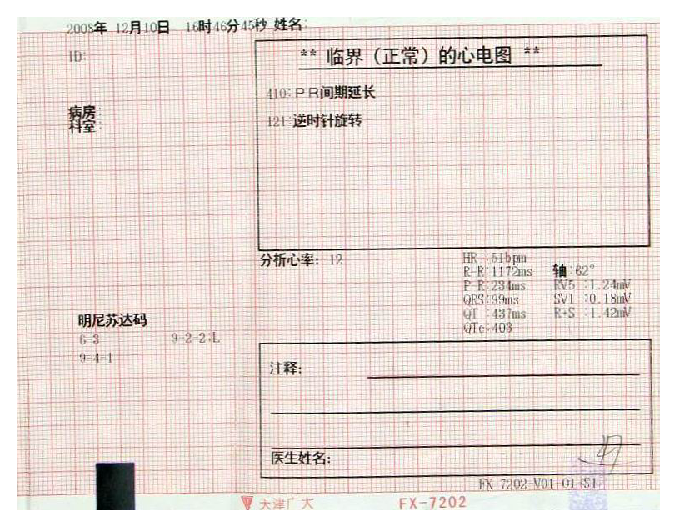
\epsfig{file=figure/f2.eps, width=0.24\columnwidth}
}
%\hfill
\subfloat[Format 3]{
\label{fig:dataset:3}
\epsfig{file=figure/f3.eps, width=0.24\columnwidth}
}
\subfloat[Format 4]{
\label{fig:dataset:4}
\epsfig{file=figure/f4.eps, width=0.24\columnwidth}
}
\caption{Examples of Four Kinds of ECGs}
\label{fig:dataset}
\end{figure}

\begin{table}[th]
\centering
\caption{Statistics for The Dataset}
\label{tab:statis}
\begin{tabular}{|c|c|c|c|c|}
\hline
Format & 1 & 2 & 3 & 4\\
\hline \hline
Number of Images & 124 & 113 & 102 & 97\\ 
\hline
Number of Attributes per Image & 17 & 16 & 18 & 15 \\
\hline
\end{tabular}
\end{table}

As the examples shown, these ECG images are in different colors 
and have many noises like grid lines. 
Because these variations and noises affect the performance of the OCR engine, 
we preprocess the images into a clean version. 
The detailed techniques are discussed in \secref{sec:discuss}. 

% we use auto thresholding to 
% preprocess the images to remove the noisy lines and 
% turn the color images into black and white. 
% An example of the preprocessing result is shown in \figref{fig:preprocess}. 
% Auto thresholding is to segment the images based on the colour 
% features automatically. In our system we make use of the tool 
% ImageJ\cite{schneider2012671} to do the preprocessing.  
% \begin{figure}[ht]
% \centering
% \subfloat[Before Preprocessing]{
% \label{fig:preprocess:1}
% \epsfig{file=figure/f1.eps, width=0.48\columnwidth}
% }
% % \hfill
% \subfloat[After Preprocessing]{
% \label{fig:preprocess:2}
% \epsfig{file=figure/pref1.eps, width=0.48\columnwidth}
% }
% \caption{Results of Preprocessing}
% \label{fig:preprocess}
% \end{figure}

\subsection{Extraction Accuracy}
Next, we compare our method with three competing methods.
The first and most naive method for information extraction from medical images 
is to write a simple parser for the XML results of the OCR engine. 
We consider this approach to be the baseline for 
evaluation. In this parser, we didn't include any fuzzy matching 
strategies, but instead extracted all results using exact matches. 

The second competing method involves marking all zones of interest 
on images and getting all the OCR results in them. 
To adjust the small changes of 
zone areas between images, a marker zone is set so that 
all other zones of interest can be adjusted against it as
a reference point. 
An example image after being marked with the zones of interest 
and the marker zone is shown in \figref{fig:zOCR} (Zones of interest 
are in blue and the marker zone is in red).

\begin{figure}[th]
\begin{minipage}{0.5\columnwidth}
\centering
\epsfig{file=figure/17_zOCR.eps, width=0.7\columnwidth}
\caption{Image Marked With Zones}
\label{fig:zOCR}
\end{minipage}
\begin{minipage}{0.5\columnwidth}
\centering
\epsfig{file=figure/17_pl.eps, width=0.7\columnwidth}
\caption{Page Layout Analysis Result}
\label{fig:pl}
\end{minipage}
\end{figure}

The third approach is to use the page layout analysis 
technique \cite{o1993document}. 
This method is used to determine where the text 
resides on a page. 
By this method, the hierarchy of physical components 
can be generated against which we can match the predefined 
hierarchy of logical components. An example result of our page layout 
analysis is shown in \figref{fig:pl}.

\begin{figure}[th]
\centering
\epsfig{file=figure/2_pl.eps, width=0.5\columnwidth}
\caption{An Error Page Layout Analysis Result}
\label{fig:errorpl}
\end{figure}


The results of comparison are shown in \tabref{tab:compare}. 
We only calculated the accuracies for extracting the results of 
variables since we already know the exact values of constant 
expressions. Based on our experiment, our method of fuzzy matching 
outperforms all other methods on all 4 types of ECGs. 
The reason is that zonal OCR and page layout analysis are highly 
related to image processing in order to extract data. The accuracy of 
zonal OCR is greatly affected by the setting of zones of interest. 
If the zones of interest are too large, it's possible that noises are
also extracted; while if the zones of interest are too small, results 
can be incomplete. For page layout analysis, the accuracy is 
affected by the granularity of the page layout unit and the 
misrecognition affects the matching with the predefined 
hierarchy of logical components. For our method, the smallest 
unit is word in text so our description can be very accurate. 
At the same time, the fuzzy matching strategies also enable 
the description to omit some unnecessary details.
% \KZ{Need focus on explaining why we are only slightly better, and what are
% the problems of the other three methods, despite that their accuracies are
% not that bad! e.g., efforts to mark the zones, I'm still not convinced
% how come without fuzzy match, zonal methods can be so good since the dist
% between the marker zone and the interesting zones can be slightly off in each
% image.}   

Even though the two competing approaches seem just marginally outperformed
by our fuzzy matching approach, these two approaches have their own 
important limitations. 
In a zonal OCR, it's important to adjust the zones of interest 
based on the marker zone. Misrecognition of the marker 
is disasterous, as all the extracted information will be incorrect. 
The other approach, page layout analysis, requires analyzing 
the text boxes in images before conducting logical labeling. 
If the text boxes are recognized incorrectly, some of the
important information may be omitted from output. 
As shown in \figref{fig:errorpl}, 
text box recognition errors cause the OCR to overlook the unit and 
other valuable information. 
However, the fuzzy match design of our system can 
tolerate these types of errors that the OCR engine often makes. 
We seek to find an optimized solution which can extract 
correct information as much as possible. 


\begin{table}[th]
\centering
\caption{Accuracy For Different Methods}
\label{tab:compare}
\begin{tabular}{|c|c|c|c|c|}
\hline
Format & 1 & 2 & 3 & 4\\
\hline \hline
Exact Match & 58.8\% & 56.3\% & 61.1\% & 53.4\% \\
\hline
Zonal OCR & 81.2\% & 79.8\% & 81.7\% & 80.6\% \\
\hline
Page Layout & 79.7\% & 80.2\% & 81.2\% & 81.1\% \\
\hline
Our Fuzzy Match & {\bf 85.5\%} & {\bf 83.8\%} & {\bf 84.9\%} & {\bf 84.0\%}\\ 
\hline
\end{tabular}
\end{table}

\subsection{Incremental Manual Correction}
%In this section, we compare the performance of 
%the human correction part in our system. 
%Another important part of our system is the human correction 
%process. By making use of the human power, we can correct 
%the errors that occur due to the OCR engine. 
We compare the two policies for recommending errors for manual correction, 
namely, random recommendation and most frequent error 
description element recommendation. The relationship between the 
amount of corrections and the accuracy of different types of 
ECGs are shown in \figref{fig:humancorr}. 
%For random correction, we randomly suggest that some errors be 
%corrected each time. 
%The accuracy of random correction is calculated by averaging 
%the results 100 times. For the most frequent error 
%description element recommendation, 
%corrections for most frequently made errors will be suggested first. 

%\KZ{Some of the words are incorrectly displayed in the following figures.}

\begin{figure}[!ht]
\centering
\subfloat{
%% \label{fig:hc:1}
\epsfig{file=figure/hcf1.eps, width=0.48\columnwidth}
}
% \hfill
% \centering
\subfloat{
% \label{fig:hc:2}
\epsfig{file=figure/hcf2.eps, width=0.48\columnwidth}
}
\hfill
% % \centering
\subfloat{
% \label{fig:hc:3}
\epsfig{file=figure/hcf3.eps, width=0.48\columnwidth}
}
% % \centering
\subfloat{
% \label{fig:hc:4}
\epsfig{file=figure/hcf4.eps, width=0.48\columnwidth}
}
\caption{Comparison of Two Correction Strategies in 4 Types of Images}
\label{fig:humancorr}
\end{figure}

% \KZ{Need to modify the figs so that lines don't touch into
% the legends, ad the caption don't overlap with the figs.}

As shown in \figref{fig:humancorr}, the more corrections we make, 
the better accuracy we get. 
The improvement to the accuracy rate is better 
when using the most frequent recommendation, compared with random 
recommendation. Using the most 
frequent recommendation is more effective, 
since we can correct more errors than random recommendation. 
With more corrections made, the improvement of 
accuracy tends to saturate, especially with regard to the 
most frequent error strategy. This is the effect of diminishing
returns, as corrections learned later tend to be minor ones and make
less impact to the overall performance.
% \KZ{Need to explain why there's only limited improvement after 15 corrections.
% Maybe because the data size is not big enough, so there's not many repeated
% errors?}
The improvement of accuracy is limited after 15 corrections. 
The main reason is that there are not many repeated errors due to 
the small size of the data set and furthermore, our system 
can only make corrections according to the correction model, 
which is sensitive to repeated errors.

% \begin{enumerate}
% \item Compare the description code with generated code to show our language is a simple one;
% \item Compare the accuracy with baseline, exact match on the OCR results, to show our language can tolerate the noises and errors;
% \item Compare the performance on different image formats;

% \item Compare the accuracy between our approach and others, including using related image position;


% \item Experiments about the relationship of the accuracy rate 
% and the number of errors corrected;

% \begin{table}[!hbp]
% \centering
% \caption{Most Frequent}
% \begin{tabular}{|c|c|c|c|c|}
% \hline
% Type & 1 & 2 & 3 & 4\\
% \hline
% Accuracy(0 errors) & 85.5\% & 83.8\% & 84.9\% & 84.0\%\\ 
% \hline
% Accuracy(1 errors) & 85.7\% & 84.0\% & 85.0\% & 84.2\%\\ 
% \hline
% Accuracy(5 errors) & 86.2\% & 84.6\% & 85.6\% & 84.8\% \\
% \hline
% Accuracy(10 errors) & 86.6\% & 85.2\% & 86.2\% & 85.5\% \\
% \hline
% Accuracy(15 errors) & 86.8\% & 85.7\% & 86.6\% & 85.9\% \\
% \hline
% % \caption{Most Frequent}
% \end{tabular}
% \end{table}

% 0 85.5 85.5
% 1 85.7 85.5
% 5 86.2 85.7
% 10 86.6 86.0
% 15 86.8 86.2

% 0 83.8 83.8
% 1 84.0 83.9
% 5 84.6 84.1
% 10 85.2 84.4
% 15 85.7 84.7

% 0 84.9 84.9
% 1 85.0 84.9
% 5 85.6 85.1
% 10 86.2 85.4
% 15 86.6 85.7

% 0 84.0 84.0
% 1 84.2 84.1
% 5 84.8 84.4
% 10 85.5 84.7
% 15 85.9 85.1

% \begin{table}[!hbp]
% \centering
% \caption{Random}
% \begin{tabular}{|c|c|c|c|c|}
% \hline
% Type & 1 & 2 & 3 & 4\\
% \hline
% Accuracy(0 errors) & 85.5\% & 83.8\% & 84.9\% & 84.0\%\\ 
% \hline
% Accuracy(1 errors) & 85.5\% & 83.9\% & 84.9\% & 84.1\%\\ 
% \hline
% Accuracy(5 errors) & 85.7\% & 84.1\% & 85.1\% & 84.4\% \\
% \hline
% Accuracy(10 errors) & 86.0\% & 84.4\% & 85.4\% & 84.7\% \\
% \hline
% Accuracy(15 errors) & 86.2\% & 84.7\% & 85.7\% & 85.1\% \\
% \hline
% % \caption{Random}
% \end{tabular}
% \end{table}


% \begin{figure}
% \centering
% \subfloat[ECG1]{
% \label{fig:hcre:a}
% \epsfig{file=figure/f1.eps, width=0.48\columnwidth}
% }
% \hfill
% \subfloat[ECG2]{
% \label{fig:hcre:b}
% 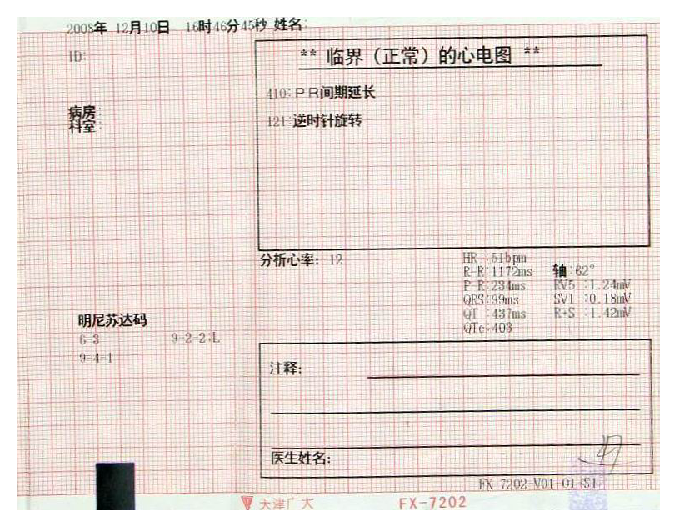
\epsfig{file=figure/f2.eps, width=0.48\columnwidth}
% }
% \hfill
% \subfloat[ECG3]{
% \label{fig:hcre:c}
% \epsfig{file=figure/f3.eps, width=0.48\columnwidth}
% }
% \hfill
% \subfloat[ECG4]{
% \label{fig:hcre:d}
% \epsfig{file=figure/f4.eps, width=0.48\columnwidth}
% }
% % \caption{E}
% \label{fig:hcre}
% \end{figure}

% \item Compare different strategies for correcting errors, including most frequent error elements, most frequent error types.
% \end{enumerate}

\section{Discussion}
\label{Discussion}



\section{Related Work}
\paragraph{Clarification Question Generation} The concept of CQ can be naturally raised in a dialogue system where the speech recognition results tend to be erroneous so that we raise CQs for sanity check \citep{stoyanchev2014towards}, or the intents for a task is incomplete or ambiguous in a first short utterance and further CQs are needed to fill in the slots \citep{dhole2020resolving}. The concept is then extended to IR to clarify ambiguous queries \citep{aliannejadi2019asking}, and has been successfully put into practice \citep{zamani2020generating}. Other application areas including KBQA \citep{xu2019asking} and open-domain dialogue systems \citep{aliannejadi2020convai3}. CQGen can also be applied to help refine posts on websites like StackExchange \citep{Kumar_2020} and Amazon \citep{rao2019answer}. In this context, our work closely follows the research line of \citep{rao2018learning, rao2019answer, cao2019controlling}. \citet{rao2018learning} first adopted a retrieval-then-rank approach. They \citep{rao2019answer} then proposed a generation approach to train the model to maximize the utility of the hypothetical answer for the questions with GAN, to better promote specificity. \citet{cao2019controlling} propose to control the specificity by training on data with explicit indicator of specificity, but it requires additional specificity annotation. Towards the similar specificity goal, we adopted a different keyword-based approach. They also assume generating one question per context, which we claim is not sufficient to cover various possible information needs, and thus propose the task of the diverse CQGen.

\paragraph{Diverse Generation} The demand for diverse generation exists in many other fields~\cite{vijayakumar2018diverse, LiangZ18code, shen2019mixture}, and we've drawn inspirations from these literatures. For image captioning, we may use multiple descriptions for different focusing points of a scene. \textit{Diverse Beam Search} \citep{vijayakumar2018diverse} was proposed to broaden the searching space to catch such diversity by dividing groups in decoding and imposing repetition penalty between them. For machine translation, a context can be translated with different styles. \citet{shen2019mixture} thus proposed \textit{Mixture of Expert} models including hMup to reflect various styles with a discrete latent variable (\textit{expert}). And here for CQGen, diversity is required to cover various potentially missing aspects, so we come up with the idea to use keywords as a controlling variable like \textit{expert} to promote diversity.


\section{Conclusion}

In this paper, we incorporated the idea of Cookie Theft picture description task into the evaluation of the high-level cognitive abilities of LVLMs and designed a novel evaluation benchmark called CogBench.
% Images in CogBench are of high quality and require more cognitive reasonings to understand, which makes it different from existing image datasets.
The images in CogBench are of high quality and demand more complex cognitive reasoning for interpretation, setting it apart from existing image datasets.
% It consists of a image description task and a VQA task.
Experiments show that there is still a large gap between the cognitive abilities of LVLMs and human beings, indicating CogBench is a challenging benchmark.

% In the future


\section*{Acknowledgments}
Kenny Q. Zhu and Jia Wei are the corresponding authors. This work
was partially supported by the AstraZeneca-SJTU collaborative
research grant.

%% main text
% \section{}
% \label{}

%% The Appendices part is started with the command \appendix;
%% appendix sections are then done as normal sections
%% \appendix

%% \section{}
%% \label{}

%% If you have bibdatabase file and want bibtex to generate the
%% bibitems, please use
%%
\bibliographystyle{elsarticle-num-names}
\bibliography{ocr}

%% else use the following coding to input the bibitems directly in the
%% TeX file.

% \begin{thebibliography}{00}
%
% %% \bibitem{label}
% %% Text of bibliographic item
%
% \bibitem{}
%
% \end{thebibliography}
\end{document}
\endinput
%%
%% End of file `elsarticle-template-num.tex'.
